\documentclass[10pt,twocolumn,letterpaper]{article}

% \usepackage{cvpr}
\usepackage{times}
\usepackage{epsfig}
\usepackage{graphicx}
\usepackage{amsmath}
\usepackage{amssymb}
\usepackage{makecell}

% Include other packages here, before hyperref.
\usepackage{subfig}
\newcommand{\subsubfloat}[2]{%
  \begin{tabular}{@{}c@{}}#1\\#2\end{tabular}%
}

% If you comment hyperref and then uncomment it, you should delete
% egpaper.aux before re-running latex.  (Or just hit 'q' on the first latex
% run, let it finish, and you should be clear).
\usepackage[breaklinks=true,bookmarks=false]{hyperref}
\usepackage{multirow}
\DeclareMathOperator*{\argmin}{argmin}
\DeclareMathOperator*{\argmax}{argmax}


\begin{document}
%%%%%%%%% Preface
\onecolumn
\pagenumbering{gobble}
% \chapter{Preface}


Transferring pre-trained representations is widely adopted by convolutional neural networks for semantic segmentation because the training data is often available only on a small scale.
In domains where directly adapting classification networks is challenging, we propose to train representations with segmentation datasets containing mislabeled objects and unsegmented objects.
Our experiments demonstrate that both mislabeled segments and incomplete segmentation lower the fine-tuning performance of the learned representations.
To get rid of the negative effect of objects label noises, we propose to assign objects of any categories a foreground label instead of the exact object categories.
Learning representations by segmenting foreground and background turns out to improve the fine-tuning performance significantly when label noises are dominant in the pre-training data.
In the existence of unsegmented objects, a sigmoid loss for the background class is proposed to achieve high recall while keeping the precision better than simply weighting the classes.
The proposed class dependent, sigmoid loss achieves both better pre-training performance and better fine-tuning performance than the class-weighted loss in the presence of incomplete segmentation.


Members of the thesis committee include Prof. dr. A.Hanjalic (Multimedia Computing Group, TU Delft) as the chair, dr. J.C. van Gemert (Vision Lab, TU Delft) who was the daily supervisor of the student, and Prof.dr. M. Loog  (Pattern Recognition Laboratory, TU Delft) and dr. Z. Szlávik (CAS Benelux, IBM).

I sincerely appreciate the magnificent supports provided by dr. J.C. van Gemert, Prof.dr. M. Loog and dr. Z. Szlávik as co-supervisors day to day.
I would also like to thank dr. D.M.J. Tax for his expert knowledge in the domain.

\begin{flushright}
{\makeatletter\itshape
    Jihong Ju \\
    Delft, \today
\makeatother}
\end{flushright}


%%%%%%%%% TITLE
\twocolumn
\pagenumbering{arabic}
\newpage
\title{Learn transferable representations in the presence of noisy labels for segmentation}

\author{Jihong Ju\\
Faculty of Electrical Engineering, Mathematics and Computer Science \\
Mekelweg 4, 2628 CD Delft\\
{\tt\small j.ju@student.tudelft.nl}
% For a paper whose authors are all at the same institution,
% omit the following lines up until the closing ``}''.
% Additional authors and addresses can be added with ``\and'',
% just like the second author.
% To save space, use either the email address or home page, not both
% \and
% Second Author\\
% Institution2\\
% First line of institution2 address\\
% {\tt\small secondauthor@i2.org}
}

\maketitle
%\thispagestyle{empty}


%%%%%%%%% ABSTRACT
\begin{abstract}

Transferring pre-trained representations is widely adopted by convolutional neural networks for semantic segmentation because the training data is often available only on a small scale.
In domains where directly adapting classification networks is challenging, we propose to train representations with segmentation datasets containing mislabeled objects and unsegmented objects.
Our experiments demonstrate that both mislabeled segments and incomplete segmentation lower the fine-tuning performance of the learned representations.
To get rid of the negative effect of objects label noises, we propose to assign objects of any categories a foreground label instead of the exact object categories.
Learning representations by segmenting foreground and background turns out to improve the fine-tuning performance significantly when label noises are dominant in the pre-training data.
In the existence of unsegmented objects, a sigmoid loss for the background class is proposed to achieve high recall while keeping the precision better than simply weighting the classes.
The proposed class dependent, sigmoid loss achieves both better pre-training performance and better fine-tuning performance than the class-weighted loss in the presence of incomplete segmentation.

% % Noisy data exists
% % Transfer learning
% % Noises affect feature transferability
% % Binarizing classes
% % Modify loss for incomplete segmentation
%
% In some domains of interest, there exist noisy segmentations in addition to a limited amount of perfect segmentations.
% Noisy segmentations can, for instance, come from crowdsourcing platforms.
% The existence of noisy datasets motivates us to consider if it is possible to utilize noisy segmentations in training better image segmentation models with limited training samples.
% We focus on to pre-train robustly transferable feature representations with potentially incomplete, mislabeled segmentations.
% In this paper, we investigate the influence of these segmentation noises on model transferability in an experimental setup with synthesized noises.
% With observing a negative impact of objects mislabeling on feature transferability, we discover that combining object categories as one foreground class improves feature transferability for a small training set corrupted heavily with random labels.
% Besides, a sigmoid loss for the background class is proposed to balance precision and recall when training with incomplete segmentations.
% % Compared to simply changing class weights, the proposed sigmoid loss down-weights the losses for confident predictions and unconfident predictions differently.
% Experiments demonstrate that replacing the cross-entropy loss with a sigmoid loss for the background class achieves better pre-training and fine-tuning performances in the presence of incomplete segmentation.
%

\end{abstract}

%%%%%%%%% BODY TEXT

\section{Introduction}
\label{introduction}

%%%%%%%%%%%%%%%%%%%%%%%%%%%%%%%%%%%%%%%%%%%%%%%%%%%%%%%%%%%%%%%%%%%%%%
%%%%%%%% TEXT Why transfer learning?
%%%%%%%%%%%%%%%%%%%%%%%%%%%%%%%%%%%%%%%%%%%%%%%%%%%%%%%%%%%%%%%%%%%%%%

% \noindent \textit{Why transfer learning? \\
% Segmentation model benefits from transfer learning.
% \begin{itemize}
%   \item Success of CNN benefits from large-scale data whereas segmentation datasets are small
%   \item Collecting segmentation in one domain on a large scale can be difficult.
%   \item One can transfer pre-trained CNN model to train with limited training samples access.
% \end{itemize}
% }

The state-or-the-art convolution neural nets benefits from transferring weights from convolutional neural network (CNN) models trained with a subset of images from ImageNet, referred to as the \textit{ImageNet models}.\cite{long2015fully,chen2016deeplab,he2017mask}
These ImageNet CNN models\cite{krizhevsky2012imagenet,simonyan2014very,szegedy2015going,he2016deep} trained for object recognition task benefit from the availability of a large-scale supervised dataset, the ILSRVC dataset\cite{russakovsky2015imagenet} which contains around 1.2 million labeled images.
In contrast to object recognition tasks, it is difficult to collect a dataset for semantic segmentaiton on that large scale.
This difficulty is natural because it costs much more efforts for people to segment than to classify an image.
Therefore, scales of semantic segmentation datasets are normally much smaller than object recognition dataset.
For instance, one of the largest segmentation datasets, Microsoft COCO2014\cite{lin2014microsoft}, contains 123,287 images for 80 object categories, smaller than the ILSRVC dataset by a factor of 10 approximately.
% the Pascal VOC2012 challenge\cite{everingham2015pascal} provides a segmentation dataset with only 9,993 segmented images for 20 object categories;
% The PASCAL-context Dataset\cite{mottaghi2014role} enriches the PASCAL VOC dataset by segmenting all 11,530 training images for 540 categories;
Therefore, semantic segmentation models are often trained with constraints of limited numbers of available training images.
A commonly used method for improving segmentation performance in the limitation of lacking training samples is to transfer weights from the pre-trained ImageNet models.\cite{long2015fully,chen2016deeplab}


%%%%%%%%%%%%%%%%%%%%%%%%%%%%%%%%%%%%%%%%%%%%%%%%%%%%%%%%%%%%%%%%%%%%%%
%%%%%%%% TEXT Why pre-training with segmentation?
%%%%%%%%%%%%%%%%%%%%%%%%%%%%%%%%%%%%%%%%%%%%%%%%%%%%%%%%%%%%%%%%%%%%%%

% \noindent \textit{Why pre-training with segmentation? \\
% ImageNet models have limitations.
% \begin{itemize}
%   \item Disimilarity in domain of interest for training images
%   \item Architecture limitation of ImageNet models. (3D ConvNet)
% \end{itemize}
% }

However, there can be limitations for these ImageNet models to significantly improve performance for a segmentation model.
Firstly, the ImageNet models were trained with relatively low resolution natural images.
In some domains of interest, training images can be non-natural, for example, aerial images, images from bird's eye view, and medical images;
In other domains, mages may have different lighting conditions from the ImageNet images such as photos taken in a dark warehouses;
Images to be segmented may also have higher resolution than the ImageNet ones.
To train a segmentation model in these domains, it can be beneficial to fine-tune the ImageNet model using a similar dataset in the domain of interest if there exists one.
Secondly, the ImageNet models cannot be applied directly to RGB-D images or 3D images like CT scans and MRI scans in 3D.
Lastly, segmentation models may have different design thinkings from classification models due to the inherent differences of the two tasks.
For example, features' translation invariance and reduced resolution for object recognition CNN models can reduce localization accuracy for segmentation.\cite{zheng2015conditional,chen2016deeplab}
The challenges in adapting ImageNet models for segmentation tasks can result in different architectures for segmentation models\cite{zheng2015conditional}.
% Even adapted segmentation models\cite{long2015fully,chen2016deeplab,he2017mask} have components not from the original ImageNet models.
Therefore, a model pre-trained with segmentation datasets in a similar domain can be useful to achieve good segmentation performance with a small training set.

% \footnote{The KITTI Vision Benchmark Suite http://www.cvlibs.net/datasets/kitti/}

%%%%%%%% ? Deeplab https://arxiv.org/pdf/1606.00915.pdf
%%%%%%%% In particular we consider three challenges in the application of DCNNs to semantic image segmentation: (1) reduced feature resolution, (2) existence of objects at multiple scales, and (3) reduced localization accuracy due to DCNN invariance.
%%%%%%%% ? CRFasRNN http://www.robots.ox.ac.uk/~szheng/papers/CRFasRNN.pdf
%%%%%%%% Firstly, traditionalCNNs have convolutional filters with large receptivefields and hence produce coarse outputs when restructured to produce pixel-level labels [37]
%%%%%%%% Secondly, CNNs lack smoothness constraints that encourage label agreement between similar pixels, and spatial and appearance consistency of the labelling output


%%%%%%%%%%%%%%%%%%%%%%%%%%%%%%%%%%%%%%%%%%%%%%%%%%%%%%%%%%%%%%%%%%%%%%
%%%%%%%% TEXT Why labels are noisy?
%%%%%%%%%%%%%%%%%%%%%%%%%%%%%%%%%%%%%%%%%%%%%%%%%%%%%%%%%%%%%%%%%%%%%%

% \noindent
% \textit{Why labels are noisy?
% \begin{itemize}
%   \item Crowd-sourcing data is noisy by nature.
%   \item ``gold standard'' itself can be ambiguous.
%   \item There exists free available noisy segmentation datasets
% \end{itemize}
% }

The pre-training segmentation datasets may, however, contain label noises, and the existence of segmentaion noises should not magnificently affect the transferability of pre-trained weights.
The use of crowd-sourcing platform like Mechanical Turk is common nowadays to collect datasets on a large scale.
However, it is natural for crowd-sourcing workers to make mistakes as a result of lack of expertise, inherent ambiguity of tasks or unconscious bias.
Enormous efforts are required, according to \cite{lin2014microsoft,everingham2015pascal}, to ensure the correctness of segmentations.
A slight decrease in percentage of segmentation errors, such as from 1\% to 0\%, may require extraordinary extra efforts due to the difficulty of identifying errors.
If not requiring ``gold standard'' segmentations, the efforts saved for correctness can be made for segmenting more images so that the result segmentations can be larger in numbers though traded with the existence of label noises.
% Trade-offs need to be made between the impact of by label noise and the gain of a larger dataset.
In some domains, for example medical imaging, the ``gold standard'' itself can be ambiguous and cause disagreements among experts.
\footnote{M: But that's OK or not?  This is what probabilities solve...}
Besides, freely available labels may exist for particular tasks, as alternatives to manual annotations.
But these labels often contain structural noises depending on the way they were created.
For example, one can use digital maps, like OpenStreetMap, to segment aerial images.
These segmentations constructed from maps would suffer from the incomplete annotation as well as registration problems.\cite{mnih2012learning}
% Besides, Pl@ntNet\footnote{https://identify.plantnet-project.org/}, a crowdsourcing platform, provide millions of images of plants and corresponding labels which may or may not be correct.
Ideally, the use of these noisy datasets for pre-training should not affect the result weights transferring to another dataset.
If negative influences of label noises on weights transferability were remarkable, methods of compensating the noises then become relevant.


%%%%%%%%%%%%%%%%%%%%%%%%%%%%%%%%%%%%%%%%%%%%%%%%%%%%%%%%%%%%%%%%%%%%%%
%%%%%%%% TEXT What types of noises exist and motivate them?
%%%%%%%%%%%%%%%%%%%%%%%%%%%%%%%%%%%%%%%%%%%%%%%%%%%%%%%%%%%%%%%%%%%%%%

% \noindent \textit{What types of noises exist and motivate them?
% \begin{itemize}
%   \item Inexaustive segmentation
%   \item Misclassification
%   \item False segmentations
% \end{itemize}
% }

\paragraph{Segmentation noises}
Noises of different kinds can exist in segmentation labels, for example, inexaustive segmentation, misclassification of segments, false segmentating, over-segmenting, under-segmenting, etc.
In particular, we consider only noises happen to labels for the whole segments instead of individual pixels, assuming the outline of segments are always correct.
That leaves us three types of noises: inexaustive segmentation, misclassification and false segmentation.
Inexaustive segmention, i.e., there exists objects left unsegmented, is one of the most frequent noises.
A typical situation of inexaustive segmentation is when images contain huge amounts of objects of the same kind, e.g. a flock of sheeps or a pile of products.
Misclassfication of segments can be avoided to some extent by asking annotators to segment one category at a time.\cite{lin2014microsoft}
Occasional misclassified objects may nevertheless still exist because of the ambiguity of category definations, for example, the misclassified bears and teddy bears in the Microsoft COCO dataset.
False segmentation denotes objects not of interest wrongly segmented as objects of interest.
It may occur due to unclear category defination, the lack of knowledge or simply visual bias.
We synthesized these three types of noises with a well-annotated dataset and studied their influences to the trained weights transferability separately.


%%%%%%%%%%%%%%%%%%%%%%%%%%%%%%%%%%%%%%%%%%%%%%%%%%%%%%%%%%%%%%%%%%%%%%
%%%%%%%% TEXT Why binarizing classes?
%%%%%%%%%%%%%%%%%%%%%%%%%%%%%%%%%%%%%%%%%%%%%%%%%%%%%%%%%%%%%%%%%%%%%%

% \noindent \textit{Why binarizing classes?}

{TODO}
Success of RPN

%%%%%%%%%%%%%%%%%%%%%%%%%%%%%%%%%%%%%%%%%%%%%%%%%%%%%%%%%%%%%%%%%%%%%%
%%%%%%%% TEXT Why PU learning
%%%%%%%%%%%%%%%%%%%%%%%%%%%%%%%%%%%%%%%%%%%%%%%%%%%%%%%%%%%%%%%%%%%%%%

If we consider inexhaustive segmenation only the problem becomes similar to a so-called \textit{positive and unlabelled learning} (PU learning) setup\cite{li2005learning}.
In the positive and unlabeled learning setup, the training dataset has two sets of examples: the \textit{positive (P) set}, containing only positive examples, and the \textit{unlabeled (U) set}, containing a mix of positive or negative examples.
The P set in an inexhaustively segmented dataset, is comprised of segmented pixels while the rest of the pixels construct the U set.
The main characteristic of the U set is that there is no easy way to generate reliable negative labels out of it so that the traditional semi-supervised learning techniques are not applicable as a result of the absence of negative training samples.
The set of background pixels containing unsegmented objects can fulfill this property of U set.
Learning to segment in the presence of inexhaustive segmentation can be thus considered as a learning problem with only positive examples and unlabeled examples.

% \noindent
% Experiments in Section \ref{subsec:robustness} indicates that inexhaustive segmentation can have significant negative influences on feature transferability.
% Besides, including mis-segmented objects for training can aggravate the inexhaustive segmentation problem.
% For example, the existence a mis-segmented toy dog does not mean that every toy dogs are mis-segmented.
% The other unsegmented toy dogs then become a source of inexhaustive segmentation and lead to worse fine-tuning performance as we discovered in Section \ref{sec:experiments}.
% Method to compensate inexhaustive segmentation is therefore necessary to train better transferable representation.

%%%%%%%%%%%%%%%%%%%%%%%%%%%%%%%%%%%%%%%%%%%%%%%%%%%%%%%%%%%%%%%%%%%%%%
%%%%%%%% TEXT Main contributions
%%%%%%%%%%%%%%%%%%%%%%%%%%%%%%%%%%%%%%%%%%%%%%%%%%%%%%%%%%%%%%%%%%%%%%

To summary, the main topics discussed in this thesis are:
\begin{enumerate}
  \item We investigated the influence of labels noises on feature transferability for semantic segmentation.
  \item Binarizing classes for pre-training can alleviate the effect caused by the existence of misclassification of segments.
  \item We proposed a class-dependent loss for unlabeled examples to compensate the influence of unsegmented objects of interest.
\end{enumerate}



%%%%%%%%%%%%%%%%%%%%%%%%%%%%%%%%%%%%%%%%%%%%%%%%%%%%%%%%%%%%%%%%%%%%%%
%%%%%%%% TEXT Table of contents
%%%%%%%%%%%%%%%%%%%%%%%%%%%%%%%%%%%%%%%%%%%%%%%%%%%%%%%%%%%%%%%%%%%%%%

The rest of this thesis is organized as follows:
In the next section, we summarize related works.
 % in areas of transfer learning, deep learning with noisy labels and PU learning.
In Section \ref{sec:robustness} we formulate the problem of pre-training with noisy segmentations and how to synthesize the three types segmentation noises.
We proposed the Exponential Unlabeled (EU) loss for noisy negative samples in Section \ref{sec:pulearning}.
Experiments in Section \ref{subsec:robustness} were designed to study the influences of inexhaustive segmentations, misclassification and false segmentation separately.
The proposed exponential unlabeled loss was evaluated in synthesized PU learning setups in Section \ref{subsec:pulearning}.
Discussions are included in Section \ref{sec:discussion} and conclusions are summarized in Section \ref{sec:conclusion}.
%Features learned by predicting the pixel objectness with inexaustive annotations were then validated with experiments described in Section \ref{sec:discussion}.


\section{Related works}
\label{sec:related}

% \paragraph{Semantic Image Segmentation with Deep Neural Nets}
%
% J. Long et.al.  \cite{long2015fully} defined a skip architecture to combine semantic information from a deep, coarse layer with appearance information from a shallow, fine layer to produce accurate and detailed segmentations and transfered the learned representations from the contemporray classification networks into fully convolutional networks.
% L. Chen et.al. \cite{chen2016deeplab} removed the last few max pooling layers of the CNNs and upsampled the corresponding filters to avoid the reduced feature resolution by the pooling layers. An additional fully connected Conditional Random Field (CRF) was added to refine the coarse last layer output for better localization performance.
% S. Zheng et.al. \cite{zheng2015conditional} integrate the CRFs-based probabilistic graphical modeling with CNNs in an end-to-end framework.


%%%%%%%%%%%%%%%%%%%%%%%%%%%%%%%%%%%%%%%%%%%%%%%%%%%%%%%%%%%%%%%%%%%%%%
%%%%%%%% TEXT Transfer Learning
%%%%%%%%%%%%%%%%%%%%%%%%%%%%%%%%%%%%%%%%%%%%%%%%%%%%%%%%%%%%%%%%%%%%%%

\paragraph{Transfer Learning}

%%%%%%%% What Transfer Learning for?

Weights of convolutional neural networks were proved ``transferable'' not only to another dataset, for example, interstitial lung disease (ILD) classification \cite{shin2016deep}, but also to other applications like object detection  \cite{girshick2014rich}, and semantic segmentation\cite{long2015fully}.
Transferable means initializing the model with weights from a pre-trained CNN model results in an improvement of the model performance compared to the random initialization. \cite{pan2010survey}
Yosinski et al. \cite{yosinski2014transferable} discovered that the transferability of features is correlated with feature generality, i.e., how much the feature depends on a particular category.
They also reported the weights from low-level layers of CNN models are well transferable to dissimilar categories, for example, from natural objects to human-made objects.
Because features are transferable regardless the exact categories they are trained with, we argue that binarizing or categorizing the pre-training classes is expected to have no significant influence to the transferability of the result pre-trained models.

% Given the superiority of transferring pre-trained weights and the availability of larger but noisier dataset, we learn transferable features with the noisy dataset and fine-tune the model with small dataset.


%%%%%%%%%%%%%%%%%%%%%%%%%%%%%%%%%%%%%%%%%%%%%%%%%%%%%%%%%%%%%%%%%%%%%%
%%%%%%%% TEXT Pre-training with weak supervision
%%%%%%%%%%%%%%%%%%%%%%%%%%%%%%%%%%%%%%%%%%%%%%%%%%%%%%%%%%%%%%%%%%%%%%

Apart from the supervised pre-training, one can also perform unsupervised learning to obtain pre-trained features in the absence of labeled training data, typically with auto-encoders \cite{vincent2010stacked,masci2011stacked}, deep belief networks \cite{hinton2006fast,lee2009convolutional}.
%%%%%%%% Deprecated UL in details
% The most common method is to train a generative model with either \textit{auto-encoder} variants or \textit{deep beilief networks}.
% Vincent et al. \cite{vincent2010stacked} trained multiple levels of representation robust to the corrupted inputs with stacked denoising auto-encoders.
% Masci et al. \cite{masci2011stacked} presented a stacked convolutional auto-encoder unsupervised pre-training for hierarchical feature extraction.
% Hinton et al. \cite{hinton2006fast} proposed a greedy learning algorithm to train \textit{deep belief nets} one layer at a time to train hierarchical features.
% Lee et al. \cite{lee2009convolutional} presented a \textit{convolutional deep belief network}, to learn hierachical convolutional representations.
% A few studies \cite{erhan2009difficulty,erhan2010does,bengio2012deep} highlighted the advantage of unsupervised pre-training compared to the random initialization, connecting unsupervised pre-training to a norm of regularization and a method that help disentangle the sample variations.
Though a few studies \cite{erhan2009difficulty,erhan2010does,bengio2012deep} discussed the advantage of unsupervised pre-trained features compared to random weights initialization, the difference between the two has been diminished ever since the arises of modern initialization strategies, namely Xavier initialization \cite{glorot2010understanding} and its variants.
We used random weights initialization as the lower baseline for pre-training with noisy labels.
Representations learned with supervision in the presence of label noise should at least outperform random weights because noisy information should be still better than no information.
% A proper method to learn features in the presence of label noise should at least outperform unsupervised pre-training because noisy information is still better than no information.

%%%%%%%%%%%%%%%%%%%%%%%%%%%%%%%%%%%%%%%%%%%%%%%%%%%%%%%%%%%%%%%%%%%%%%
%%%%%%%% TEXT DL with noisy labels
%%%%%%%%%%%%%%%%%%%%%%%%%%%%%%%%%%%%%%%%%%%%%%%%%%%%%%%%%%%%%%%%%%%%%%

\paragraph{Deep Learning with Noisy Labels}

The impact of randomly flipped labels on classification performance has been investigated by \cite{sukhbaatar2014training,patrini2016making} for convolutional neural networks.
They both reported decreases in classification performance as the proportion of flipped labels increases for a fixed number of training samples.
On the other hand, Rolnick et al. \cite{rolnick2017deep} argued that deep neural networks can learn robustly from noisy datasets as long as appropriate choices of hyperparameters were made.
They studied the effect of label noise by diluting correct labels with errored labels instead of corrupting correct labels with errored ones and argued that collecting more labels is of more importance than correcting the obtained labels.
None of these studies explored the influence of label noise on feature transferability.
To the best of our knowledge, we are the first research to investigate representations robustness to label noise.

To alleviate the negative effects on classification performance introduced by errored labels, a few methods were proposed for deep neural network models.
Sukhbaatar et al. \cite{sukhbaatar2014training} introduced a linear noise layer on top of the model output, and Patrini et al. \cite{patrini2016making} proposed two forms of loss correction concerning the label observation bias.
Xiao et al. \cite{xiao2015learning} integrated a probabilistic graphic model to an end-to-end deep learning system to predict the observed labels and to correct the observed labels.
Additionally, Reed \& Lee \cite{reed2014training} proposed a bootstrapping loss to emphasize \textit{perceptual consistency} when learning in the presence incomplete and errored labels.
All these methods are proposed to solve label errors from any class to any class but often have the capability of solving specific errors from one class to another.
In our problem of learning with only positive and unlabeled data, the unlabeled data can be treated as a set of examples assigned with correct negative labels and incorrect negative labels.
The problem then converts to learning in the presence of label errors from positive to negative but not from negative to positive.
We modified the bootstrapping loss to interpret the prior knowledge that positive labels are reliable, and set a benchmark in the experiments for the state-of-the-art methods.

%%%%%%%% some more methods
% To study the effect of errored labels, we simulate datasets with random flipped labels from clean labels.
% We also designed our experiments using stochastically simulated noisy segmentations from perfect segmentation.

%%%%%%%% Irrelevant
% Yosinski et al. discovered that feature transferability is negatively affected by the specialization of higher layer neurons and optimization difficulties caused by breaking co-adapted neurons.
% discovered that transferability of a feature is correlated with its generality, i.e. by how much it depends on a particular category.
% Their experiments showed that low-level features, which are less dependent to particular categories, are more transferable than high-level features.
% In general, optimal classification performance on test set often indicates that the extracted features are also optimal, whereas suboptimal classification performance does not necessarily reflect the convolutional features are also suboptimal, especially concerning feature transferability.
% Feature transferability describes the \textit{generality of features}, i.e., the category-independence of features.
% Low-level features were proved to be less dependent to categories and thus more transferable to new tasks than high-level features.  \cite{yosinski2014transferable}
% We experimented in Section \ref{sec:robustness} that how much label noises interfere the transferability of convolutional features.

% Additionally, most of these studies focus on the classification problems, whereas our work inclined more to the semantic segmentation problem.

%%%%%%%%%%%%%%%%%%%%%%%%%%%%%%%%%%%%%%%%%%%%%%%%%%%%%%%%%%%%%%%%%%%%%%
%%%%%%%% TEXT PU Learning
%%%%%%%%%%%%%%%%%%%%%%%%%%%%%%%%%%%%%%%%%%%%%%%%%%%%%%%%%%%%%%%%%%%%%%

\paragraph{Positive and Unlabeled Learning}

Traditional methods to learn with only positive samples and unlabeled samples for text classification \cite{liu2003building,li2005learning} often follow a two-step strategy: (1) first identifying a set of reliable negative samples (RN set) from U set and (2) then iteratively build a set of classifiers with RN set and P set, while updating the RN set with a selected classifier.
Methods following this two step strategy do not extend well to deep learning models because it would take tremendously longer time to iteratively train a sequence of deep learning models than to train a sequence of na\"ive Bayesian (NB) models or supported vector machines (SVMs).
For this reason, we do not consider training deep neural networks following this two-step strategy in this work.

Alternatively, one can treat all unlabeled examples as negative, and weight the losses for positive and negative examples differently \cite{lee2003learning}.
Under the assumption that which positive examples are selected to be labeled is completely at random, i.e., independent of the input features, Elkan \& Noto \cite{elkan2008learning} proved that the probability for an object of being observed as positive differs from the probability of being truely positive by a constant factor.
They also observed that a classifier trained on positive and unlabeled examples predicts probabilities that differ by only a constant factor from the true conditional probabilities of being positive.
These two works considered only binary classification.
We provide an extension of binary PU learning to multiclass PU learning where examples from multiple relevant classes are partially unlabeled and mixed with examples for the non-relevant class.

The often used logistic loss for neural networks grows to infinity as the confidence of wrong prediction increases to one.
This can be a problem for class-weighed loss: the superfluous penalty for confident, positive predictions, i.e., samples far from the decision boundary have a large influence on the final solution. \cite{tax2016class}
Du et al. \cite{du2015convex} illustrated that the logistic loss and the hinge loss perform worse than the ramp loss in the PU classification setting due to their superfluous penalty for confident predictions.
The non-convex Ramp loss \cite{du2014analysis} and a convex double hinge-loss \cite{du2015convex} were proposed separately to learn from positive and unlabeled data by Du et al.
But neither of the two losses are continuous, which is problematic for a gradient based optimization so that we turns to a continuous altenative of the ramp loss, the sigmoid loss.

Tax \& Wang \cite{tax2016class} proposed to use the sigmoid loss for the positive class to retrieve relevant objects from a large, non-relevant objects dominant dataset, with only poorly labeled relevant objects.
PU learning is happening on an opposite side of this retrieving problem: the positive examples are labeled reliably and the unlabeled examples can be considered as poorly labeled negative examples.
% Lin et al. \cite{lin2017focal} proposed a so-called Focal Loss to down-weight confident predictions and thus focus training on hard negatives for imbalanced learning.
So we proposed to use the sigmoid loss\cite{tax2016class} for the negative class to alleviate the superfluous punishment for confident, positive predictions.
% Using the sigmoid loss for the negative class only is an interpretation of the prior knowledge that the positive labels are reliable while the negative labels are not.


\section{Noise robustness of feature transferability}
\label{sec:robustness}

%%%%%%%%%%%%%%%%%%%%%%%%%%%%%%%%%%%%%%%%%%%%%%%%%%%%%%%%%%%%%%%%%%%%%%
%%%%%%%% TEXT Noise model
%%%%%%%%%%%%%%%%%%%%%%%%%%%%%%%%%%%%%%%%%%%%%%%%%%%%%%%%%%%%%%%%%%%%%%

\noindent \textit{From feature generality to feature robustness}

\noindent
The first convolutional features for images are often observed converged to either Gabor filters or color blobs even training with different datasets and different objectives\cite{zeiler2014visualizing,lee2009convolutional,krizhevsky2012imagenet,shin2016deep}.
These standard features on the first layer are called \textit{general} because they often occur independent of the exact cost function and natural image dataset.
By contrast, the last-layer features depend significantly on the given labels otherwise the training errors would be high which is against learning objective.
These features are then denoted as \textit{specific}.
As we mentioned in Section \ref{sec:related}, Yosinski et al. \cite{yosinski2014transferable} studied the features in the intermediate layers and found the weights transferability decreases from the first layer to the last layer, alongside the specificity increases from the first layer to the last layer.
Given the evidence that low-level features can be independent of a particular category, we wonder if the learned features are robustness to label noises regarding their transferability to a new task.
For instance, if some dogs were incorrectly annotated as cats in the base dataset for pre-training, would these annotation noises influence transferability of the learned features to a new task recognize or detect sheep?

\noindent
We experimented, in Section \ref{subsec:robustness}, how transferable the learned features are in the presence of three types of annotation noises: \textit{misannotation}, \textit{misclassification} and \textit{inexaustive annotation}.
We synthesized these three types of errors with the probabilitic model discussed with a well-annotated dataset and studied how the synthesized errors influence transferability of learned features compared to the noise-free cases.
Feature transferability can be evaluated by how much transferring the features improves the performance of training a new dataset compared to training with random weights initialization. \cite{yosinski2014transferable}


\subsection{Problem Formulation}
\label{subsec:formulation}

\noindent \textit{Formulation of segmentation}
\noindent
The goal of semantic segmentation tasks is to segment images into semantically meaningful partitions, a.k.a.,\textit{segments}.
These segments are \textit{target} if they depict instances of pre-defined object categories or \textit{non-target} otherwise.
A common way of interpreting semantic image segmentation tasks with CNNs is the pixel-wise classification model:
Given an image $x$, a segmenting model $f: R^{h \times w \times c} \rightarrow R^{h \times w}$ predicts a label for each pixel and output a label map $y$ that has the same size as $x$.
$h, w$ are image height and weight respectively, and $c$ is the number of image channels.
Supposing there are $K$ predefined categories, each pixel in $y$ is assigned a label $y_{ij}=k$, where $ij$ specifies the pixel with $i \in [1,h], j \in [1,w]$.
The assigned label $k \in [1, K]$ if the pixel corresponds to an instance of one of the $K$ categories; $k=0$ if the pixel is correspondent to a non-target segment.
We can also name pixels with $k=0$ as \textit{unannotated} since they were not assigned to one of the predefined categories.

\noindent \textit{Noise model}
\noindent
Noisy labels can be considered as true labels corrupted with a noise model.
The noise model describes the probabilistic distribution of the observed label map conditioning on the the true label map $y$, the image $x$ and label errorness $e$:
$$p(\tilde{y} \vert x, y, e)$$
where the occurence of errors $e$ for pixels depends on the inputs $x$ and true labels $y$.
Such a noise model is called noisy not at random (NNAR) \cite{frenay2014classification} because the noise depends on not only the true label $y$ but also the inputs $x$.

\noindent \textit{Clarity for noise considered.}
\noindent
% In the above model, label errorness for pixels is assumed to be independent to each other despite the fact that neighboring pixels are likely to have the same label in practice.
%Conditional random fields (CRF) were introduced to interpret the neighboring pixel dependence.\cite{chen2016deeplab}
All the errors considered in this work apply to the whole segment instead of to individual pixels.
This means if one pixel for an object has a wrong label, the pixels that also belong to this object will have the same wrong label.
% This can be interpreted as a probablilistic distribution of the observed label for pixel $ij$ conditioned on its true label $y_{ij}$, the image $x$, and observed labels for the other pixels $\{\tilde{y_{kl}}, kl \in P \setminus \{ij\} \}$:
% $$p(\tilde{y_{ij}} \vert x, y_{ij}, \{\tilde{y_{kl}}, kl \in P \setminus \{ij\} \})$$
% where $P$ is the set of all pixels in image $x$.
By doing so, we exlude segmenting errors such as inprecise boundaries, oversegmenting or undersegmenting the objects from discussion.
These types of errors are not the focus of our works and may lead to future studies.

% \noindent
% In general, the observed value of a pixel label $\tilde{y_{ij}}$ depends on the joint distribution of its true label $y_{ij}$, the occurence of an error $e_{ij}$, and the input image $x$, and the occurence of an error $e_{ij}$ depends on both $x$ and $y_{ij}$.
% This model is denoted as \textit{noisy not at ramdom (NNAR)}\cite{frenay2014classification}: $p(\tilde{y_{ij}},x) = p(\tilde{y_{ij}} \vert x, y, e_{ij}) p(e_{ij} \vert x,y)$.
% However, there are two difficulties estimate $p(\tilde{y})$ with the NNAR model:
% neighboring pixel dependency
% x dependency
%
% $p(\tilde{y} \vert y,e) p(e \vert y)$
% It is nevertheless difficult to fit such a NNAR model directly because it is difficult to estimate of $p(e \vert x,y)$ with limited number of samples.
% An alternatie model is the \textit{noisy at random (NAR)} model in which the occurence of errors $e$ are independent to $x$ only on $y$: $p(\tilde{y} \vert y)p(y \vert x)$
% Such \textit{Noisy at random (NAR)}

% \noindent
% The probability of obsesrving a pixel label $\tilde{y_{ij}}$ depends on inputs $x$, the true label of that pixel $y_{ij}$, and labels of the rest pixels in that image:
% $$p(\tilde{y_{ij}} \vert x, y_{ij \in P}, \{ y_{mn}: mn \in P \setminus \{ij\} \})$$

% \noindent
% where $P$ is the full set of pixels in one image and $i,m \in [1,h], j,n \in [1,w]$.



\noindent
\paragraph{Misannotation}
Misannotation denotes the errors wrongly segmenting objects of categories that are semantically meaningful but not predefined as objects of pre-defined categories.
For example, a toy dog was misannotated as a dog given that ``dog'' was predefined and ``toy dog'' was not.
These misannotated objects have pixel labels transited from $0$ to $k$ with probability $p(\tilde{y_{ij}}=k \vert x, y_{ij}=0, \{\tilde{y_{kl}}, kl \in P \setminus \{ij\} \})$, where P
We assumed that misannotation would happen to only semantically meaningful segments in images because it is less likely for partitions which have no semantical meaning to be misannotated.
Given a perfectly annotated training set, we can synthesize misannotation errors by selecting part of the categories as segmenting target and assigning the target labels to non-target segments.


\noindent
\paragraph{Misclassification}
Misclassification error means objects misclassified from one pre-defined category to another.
It is similiar to misannotation error except that both correct and incorrect classes belong to the pre-defined set of categories.
For example, cats was misclassified as dogs given that both ``cat'' and ``dog'' are target classes.
The misclassified pixels transit from $k$ to $l$ with probability $p(\tilde{y_{ij}}=l\vert x, y_{ij}=k)$, where $k,l \in [1, K]$.


\noindent
\paragraph{Inexaustive annotation}
Inexaustive annotation denotes that there exists unsegmented objects for pre-defined categories.
Pixels for the unannotated objects have labels flipped from $k$ to $0$.
$p(\tilde{y_{ij}}=0\vert x, y_{ij}=k)$, where $k \in [1,K]$



% The inexhaustive annotations need to be properly handled given the prior knowledge modeling the missing pattern of the annotations.
% Given that we believe any annotated instance provide information, all the foreground pixels that correspond to the annotated instances become reliable and the background pixels may contain both the true background pixels and object pixels unannotated.
% That satisfies a Positive and Unlabeled learning setup where the training dataset contains only the positive examples and unlabeled examples that are the mixed of the positive samples and negative samples.


\subsection{Synthesized dataset}
\label{subsec:robustness}

%%%%%%%% TEXT
\noindent
\textit{Experiment setup}
\noindent
In order to investigate the influence of misannotation, misclassification and inexaustive annotation on feature transferability, we set up experiments with the perfectly annotated dataset, PASCAL VOC2011\cite{everingham2015pascal}.
The 20 categories of VOC2011 were divided equally into four folds, and the exact partitions are listed in Table \ref{tab:objectness}.
For each fold, images were split into two set: \textit{pre-training set} consists of images with segments of the 5 target classes and \textit{fine-tuning set}  images contained only objects of the other 15 classes.
Pre-training set was used to pre-train weights and fine-tuning set was used to fine-tune the pre-trained weights.
Misannotation, misclassification and inexaustive annotation were synthesized by polluting well-annotated pre-training dataset in different manners.
Pre-trained weights learned in the presence of synthesized noises were compared against those trained with the corresponding noise-free annotations.
The transferability of learned weights were evaluated by performance achieved with the fine-tuning test set.
We used the mean intersection over union (mean IU) metric to evaluate the segmentation performance, following the VOC segmentation challenge.

\noindent \textit{Experiment details}
\noindent
To keep the segmenting task simple, we used images containing only a single object and excluded those that have multiple objects from both the pre-training set and the fine-tuning set.
The training dataset was enriched with the SBDD annotations due to the limited number of available segmentations from the official PASCAL VOC2011 dataset, resulting in 4000 training images of 20 categories in total.
In order to accelerate the training process, we subsampled the original images by four times.
Fully Convolutional Networks with AlexNet was used for experiments because its simplicity and relatively short training time and the existence of an ImageNet model for AlexNet.
Only weights of convolutional filters in AlexNet were transfered from the pre-training phase to fine-tuning phase and the other layers were random initialized, with Xavier Initialization.
By doing this, the ImageNet model and completely random weight initialization become the upper bound and lower bound respectively for various pre-trained weights summarized in Table \ref{tab:objectness}.
The default hyperparameters of FCN-AlexNet\cite{long2015fully} were kept unchanged.
Training run 240,000 iterations for pre-training phase, and 12,000 iterations for fine-tuning phase.


\noindent \textit{What Table \ref{tab:objectness} tell us.}
\noindent
Feature transferability in the presence of synthesized misannotation, misclassification and inexaustive annotation were studied seperately.

\noindent \textit{
How misannotation is synthesized;
How synthesization different from reality;
What are the result;
}
\noindent
As discussed in Section \ref{subsec:formulation}, we synthesized misannotation errors by selecting one category as target and assigning instances of the other 14 categories target labels.
The corresponding noise-free case is datasets with only the selected target category annotated and the other 14 categories unannotated.
These two cases were denoted as BinaryCategory and SingleCategory seperately in Table \ref{tab:objectness}.


Misclassification: TrueLabels vs. RandomLabels
Misclassification

Inexaustive annotation: TrueLabels vs. InexaustiveLabels

%%%%%%%% Table Learn Pixel Objectness for pre-training
\begin{table}[t]
\resizebox{\columnwidth}{!}{
\centering
\begin{tabular}{l|llll}
\makecell{Initial \\Representation}  & \makecell{mean IU \\(aerospace, bicycle, \\bird, boat, \\bottle)} & \makecell{mean IU \\(bus, car, \\cat, chair, \\cow)} & \makecell{mean IU \\ (dining table, \\dog, horse, \\motorbike, person)} & \makecell{mean IU \\(potted plant, \\sheep, sofa, \\train, TV)} \\
\hline
ImageNetModel    & \makecell{$0.42\pm0.01$} & \makecell{$0.51\pm0.01$} & \makecell{$0.49\pm0.01$} & \makecell{$0.47\pm0.01$} \\
RandomWeights    & \makecell{$0.29\pm0.01$} & \makecell{$0.29\pm0.03$} & \makecell{$0.27\pm0.01$} & \makecell{$0.30\pm0.02$} \\
\hline
SingleCategory   & \makecell{$0.26\pm0.01$} & \makecell{$0.37\pm0.03$} & \makecell{$0.27\pm0.01$} & \makecell{$0.33\pm0.04$} \\
BinaryLabels     & \makecell{$0.30\pm0.02$} & \makecell{$0.35\pm0.01$} & \makecell{$0.29\pm0.02$} & \makecell{$0.35\pm0.03$} \\
\hline
TrueLabels       & \makecell{$0.29\pm0.01$} & \makecell{$0.36\pm0.01$} & \makecell{$0.29\pm0.01$} & \makecell{$0.37\pm0.01$} \\
AllRandomLabels  & \makecell{$0.29\pm0.01$} & \makecell{$0.33\pm0.03$} & \makecell{$0.26\pm0.01$} & \makecell{$0.28\pm0.01$} \\
HalfRandomLabels & \makecell{$0.29\pm0.00$} & \makecell{$0.33\pm0.00$} & \makecell{$0.26\pm0.00$} & \makecell{$0.28\pm0.00$} \\
InexaustiveLabels& \makecell{$0.27\pm0.00$} & \makecell{$0.32\pm0.00$} & \makecell{$0.26\pm0.00$} & \makecell{$0.34\pm0.00$} \\
\end{tabular}
}
\caption{Performances of FCN with Alexnet trained with different representation initializations to segment five categories from the PASCAL VOC2011 dataset.
\textit{ImageNetModel} represents the pre-trained ImageNet model;
\textit{RandomWeights} indicates that the weights were randomly initialized with Xavier Initialization;
All the other weights were pre-trained with images of the complementary fifteen categories for the five fine-tuning target categories.
\textit{SingleCategory} was pre-trained on only one annotated category, either ``dog'' or ``cat'' depending on the fold, and the other categories were left unannotated;
\textit{BinaryLabels} was pre-trained with binary labels that any objects of the fifteen categories were annotated as one single category, namely ``dog'' or ``cat'' depending on fold;
\textit{TrueLabels} was pre-trained with all objects segmented and assigned to 15 categories correctly;
\textit{AllRandomLabels} was pre-trained with all objects correctly segmented but assigned random labels;
\textit{HalfRandomLabels} was pre-trained with all objects correctly segmented and half of them randomly assigned labels;
\textit{IncompleteLabels} was trained with datasets that objects were annotated correctly with a probability of 0.5;
}
\label{tab:objectness}
\end{table}
% Supposing a dog is wrongly annotated as a cat, the error could mislead the model to predict the dog as cat because the learning objective drives the model to fit the given labels.
% But dogs and cats have visual features: they are both furry, have similiar shape and appearance, etc.
% These similiarities in features between dogs and cats may correspond to some interm features when a toy dog was misannotated as a dog.
% If we consider further lower features, for exmaple those for detecting edges and corners, they are commonly transferable to many categories, not necessarily ones that look alike.
% dissimilar categories (man-made classes and natural classes)
%If we constraint ourselves to perceive only part of the dog and the toy dog, for example the ears, it may become difficult even for us to distinguish the two because given only the local information there is not much difference between them.
% The generality of the low-level features can introduce the robustness to misannotations regarding the transferability when we want to transfer hieraychical features for semantic segmentation in the presence misannotated objects because the low-level features are not dependent on the exact category assigned to the objects.
% This annotation error robustness for the low-level features could result in noise robustness for the multiple level pre-trained weights for semantic segmentation with noisy labels.
% In Section \ref{sec:objectness}, we tested whether object misannotation had an impact on the transfehen we transfer the learned features to a new dataset with new categories.
% That leads us to the following research question:
% \begin{enumerate}
%   \item How do misannotation and misclassification of instances influence the ``transferability'' of the learned features respectively?
% \end{enumerate}


\section{Positive and Unlabeled Learning}
\label{sec:pulearning}

\noindent \textit{This part should explain the necessarity of Positive and Unlabeled Learning setup, including the importance to make a difference between inexaustive annot. and misclassification.}

\noindent
We discussed in Section \ref{sec:robustness} that misclassification and inexaustive annotation can have negative influence on feature transferability, which is undesirable when we train transferable weights with noisy data.
Therefore, methods to compensate these errors are discussed in this section.
In practice, misclassification error is less likely to \textit{dorminate} and dorminate means the misclassified rate outperforms the correct rate.
However, unannotated objects can be dorminant for a large dataset.
Besides,
the most studied \cite{reed2014training,sukhbaatar2014training,patrini2016making,jindal2016learning}
Therefore, we focus on inexaustive annotation.

%%%%%%%% TEXT PU Learning setup
\paragraph{Formulation}
\noindent \textit{This part should formulate the problem with a probability model and make clear statement that model here is different from previous section: model to corrupt and model to recover.}
\noindent
When we synthesized errors in Section \ref{sec:robustness}, we assumed that the observed labels depend on
$p(\tilde{y} \vert x, y)$.

$p(\tilde{y_{ij}} \vert y_{ij})$.
This model is easy to apply when we have the perfect annotations and want to generate noisy labels, but it is not as easy when we observe noisy labels and want to recover the correct ones.

$p(\tilde{y_{ij}} \vert y_{ij})$


%%%%%%%% TEXT Modeling
\paragraph{Weighted Logistic Regression}
\noindent \textit{This part should discuss the linear model for observing positive conditioning on true positive and its relationship to changing the class weight.}


%%%%%%%% TEXT Exponential loss
\paragraph{Exponential Loss for unlabeled examples}
\noindent
\textit{This part should explain why the exponential loss could perform better than the cross-entropy loss, potentially with a figure of 2D Gaussians.}
The ``soft'' bootstrapping loss in \cite{reed2014training} is actually equivalent to a softmax regression with \textit{minimum entropy regularization}\cite{grandvalet2005semi} which was originally proposed for semi-supervised learning.
Minimum entropy regularization encourages the model to have a high confidence in predicting labels.

%%%%%%%% TEXT Expontial loss FADE IN

\paragraph{Implementation details}
\noindent \textit{This paragraph should explain fade-in was introduced to avoid all-positive inital prediction;}

\noindent

%%%%%%%% TEXT Imbalanced
\noindent
\textit{This part should explain the influence of the imbalanced problem and how to overcome.}



%%%%%%%% FIGURE MOONS
\begin{figure*}
\begin{center}
% \fbox{\rule{0pt}{2in} \rule{.9\linewidth}{0pt}}
   \includegraphics[width=0.95\linewidth]{img/moons.png}
\end{center}
   \caption{2D moons dataset with non-linear separable decision boudary. Four hundreds samples per class were drawn randomly from two interleaving half circles with noises added with a minor standard deviation. A \textbf{red circle} indicates an example labelled as positive whilst a \textbf{blue square} indicates the example has a negative label. The \textbf{leftmost} figures have complete positive labels, meaning the positive and negative labels are all correct, whereas, in \textbf{the other figures} only half of the positives were correctly labelled and the rest were mixed with the negative samples. The \textbf{background colors} represent the probability for the area to be positive given by the classifier trained with the given samples and labels: \textbf{red} for high probability areas, \textbf{blue} for low probability areas and \textbf{white} for the class transition areas, i.e.decision boundaries. The \textbf{size of the markers} in the top row denotes the per-class normalized training losses and the \textbf{size of the markers} in the bottom row the per-class normalized derivatives w.r.t the output of the last layer for the trained Multilayer Perceptron (MLP) with the different losses.}
\label{fig:moons}
\end{figure*}


%%%%%%%% FIGURE Losses
\begin{figure}[t]
\centering
% \fbox{\rule{0pt}{2in} \rule{0.9\linewidth}{0pt}}
   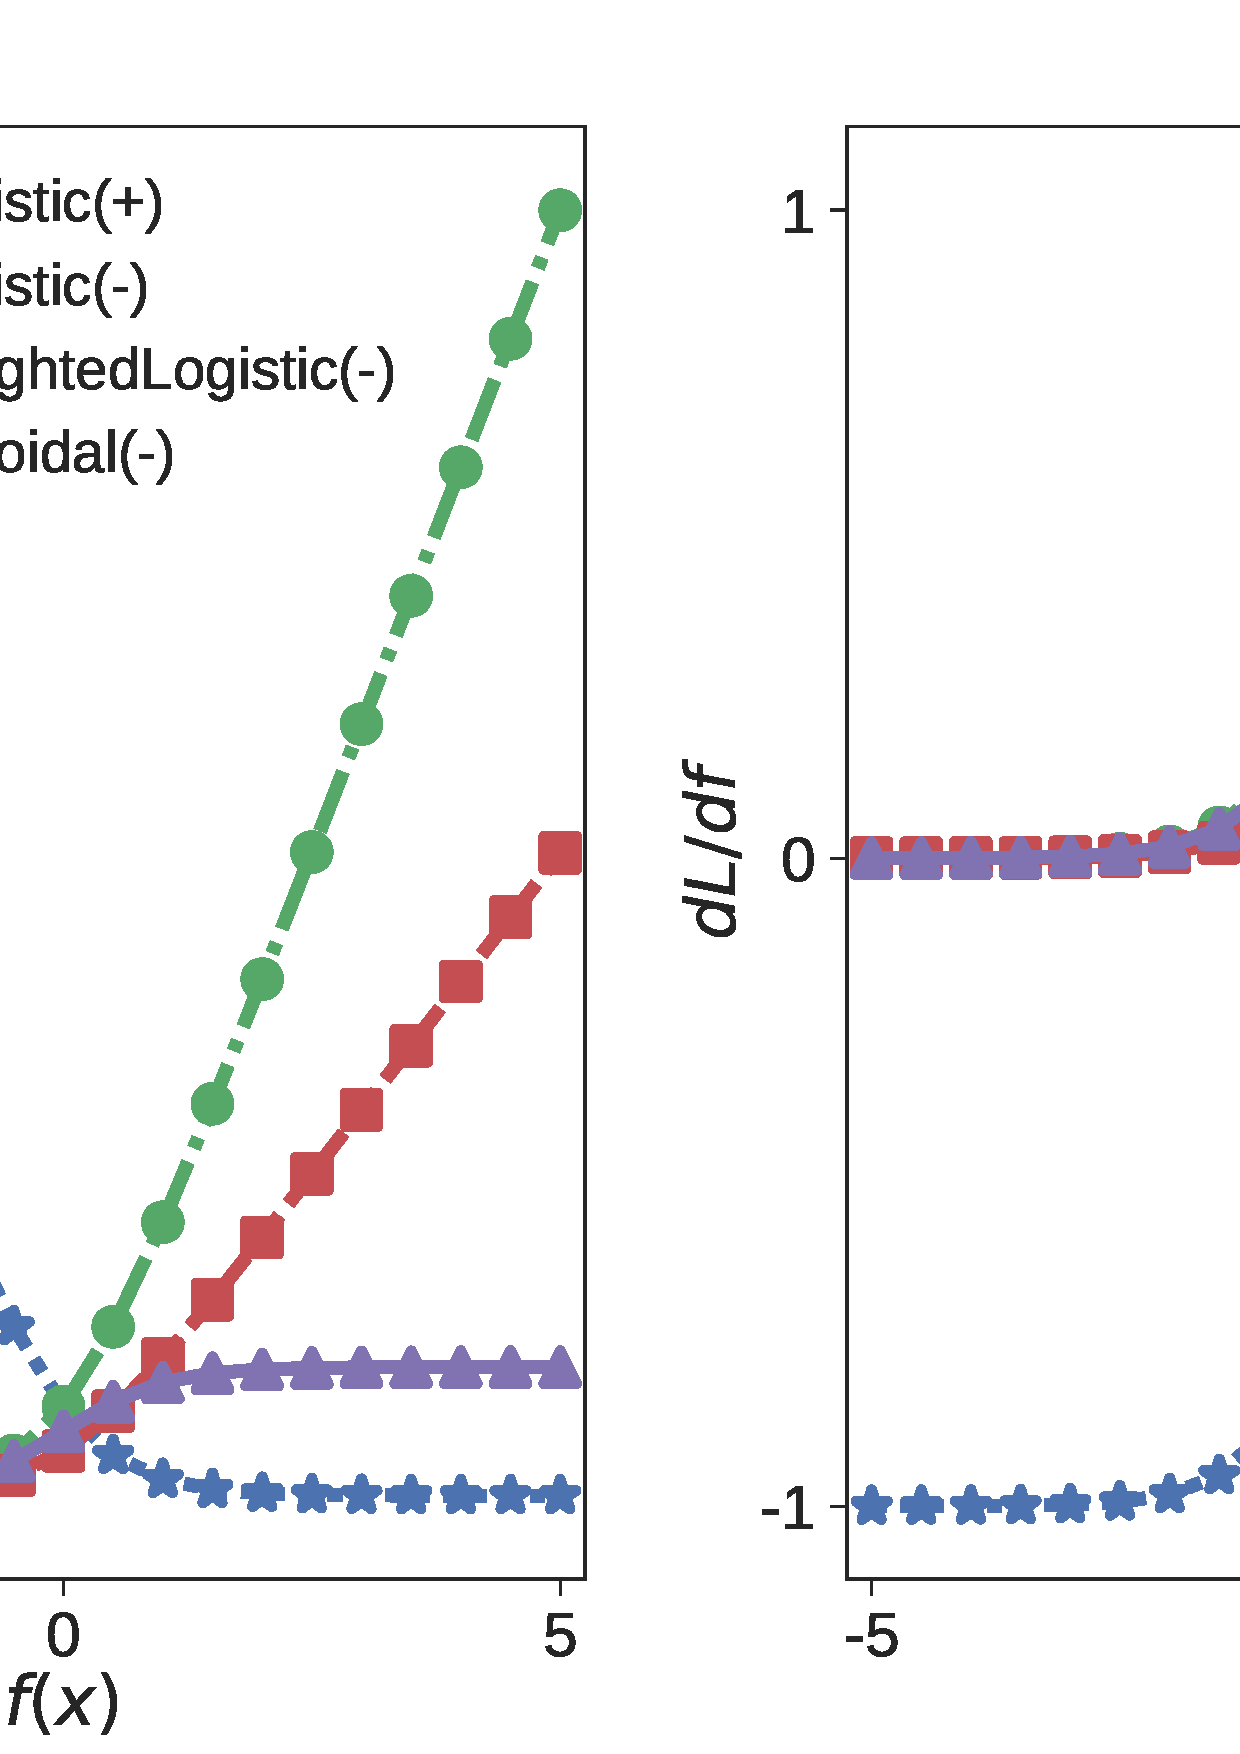
\includegraphics[width=0.95\linewidth]{img/losses.png}
\caption{The Logistic Loss, Weighted Logistic Loss, Exponential Loss and their dirivatives with respect to the model output.}
\label{fig:losses}
\end{figure}


%%%%%%%% FIGURE Varying positive annotating percetage
\begin{figure}[t]
\centering
\fbox{\rule{0pt}{2in} \rule{0.9\linewidth}{0pt}}
  %  \includegraphics[width=0.95\linewidth]{img/}
\caption{Varying percentage of annotated positives 10\%, 20\%, 50\%, 80\% and 100\% with images from CIFAR10 as the positives and images from CIFAR110 as the negatives.}
\label{fig:pct_annotating}
\end{figure}

%%%%%%%% TABLE CIFAR10
\begin{table}[t]
\resizebox{\columnwidth}{!}{
\centering
\begin{tabular}{ll|llll}
Annotation  & Loss & acc. & prec. & rec. & $F_1$ \\
\hline
Complete    & CrossEntropyU.   & $0.87\pm0.01$ & $0.88\pm0.01$ & $0.82\pm0.01$ & $0.85\pm0.01$ \\
50\%(P+N)   & CrossEntropyU.   & $0.83\pm0.01$ & $0.84\pm0.01$ & $0.78\pm0.01$ & $0.80\pm0.01$ \\
50\%P+U     & CrossEntropyU.   & $0.64\pm0.04$ & $0.93\pm0.08$ & $0.34\pm0.02$ & $0.44\pm0.06$ \\
50\%P+U     & WeightedU.       & $0.78\pm0.01$ & $0.75\pm0.01$ & $0.75\pm0.01$ & $0.76\pm0.01$ \\
50\%P+U     & ExponentialU.    & $0.82\pm0.01$ & $0.86\pm0.01$ & $0.73\pm0.01$ & $0.78\pm0.01$ \\
50\%P+U     & BootstrapHard    & $0.74$ & $0.81$ & $0.60$ & $0.67$ \\
50\%P+U     & DropoutReg.      & & & & \\
\end{tabular}
}
\caption{Image classification with positive examples partially annotated. The complete dataset contains images from CIFAR10 as the \textbf{positive} (P) set and images from CIFAR110 as the \textbf{negative} (N) set. The unannotated positive examples from P set construct the \textbf{unlabeled} (U) set together with the N set.}
\end{table}


%%%%%%%% TABLE
\begin{table}[t]
\resizebox{\columnwidth}{!}{
\centering
\begin{tabular}{ll|llll}
Annotation  & Loss & pixel acc. & mean acc. & mean IU & f.w. IU \\
\hline
Complete    & CrossEnt.U    &  &  & & \\
50\%(P+N)   & CrossEnt.U    & & & & \\
50\%P+U     & CrossEnt.U    & & & & \\
50\%P+U     & WeightedU        &  &  & & \\
50\%P+U     & ExponentialU     &  &  & & \\
50\%P+U     & BootstrapHard    &  &  & & \\
50\%P+U     & DropoutReg. & & & & \\
\end{tabular}
}
\caption{Image semantic segmentation with images contain single instance only from the PASCAL VOC2011 segmentation dataset. The complete \textbf{positive} (P) set denotes the foreground instances and the \textbf{negative} (N) set consists of the background. The unannotated instances from P set construct the \textbf{unlabeled} (U) set together with the N set.}
\end{table}


\section{Experiments}
\label{sec:experiments}

\subsection{Synthesized misannotation, misclassification and inexhaustive annotations}
\label{subsec:robustness}

%%%%%%%% TEXT
\noindent
\textit{Experiment setup}
\noindent
In order to investigate the influence of misannotation, misclassification and inexaustive annotation on feature transferability respectively, we set up experiments with a perfectly annotated dataset, PASCAL VOC2011\cite{everingham2015pascal}.
15 out of 20 categories were selected to form a \textit{pre-training dataset} and the other categories formed a \textit{fine-tuning dataset}.
The pre-training dataset was used to train Fully Convolutional Networks with AlexNet (FCN-AlexNet) models in the precense or absence of synthesized segmentation errors.
The fine-tuning dataset was used to fine-tune the weights of convolutional layers from the pre-trained FCN-AlexNet model.
The fine-tuned models were evaluated by the mean intersection over union ratio (mean IU) achieved with the test set of the fine-tuning dataset.
The performance of fine-tuning model comparing to the random-initialized model indicates transferability of the pre-trained weights,

\noindent
In order to avoid the influence of categories-splitting choice, the 20 categories of VOC2011 were divided equally into four folds and each fold was studied separately.
The exact partitions of categories are listed in Table \ref{tab:robustness}.

\noindent \textit{Experiment details}
\noindent
The training dataset was enriched with extra manual segmentations by Hariharan et al.\cite{hariharan2011semantic}
To keep the segmentation task simple, we used only single-object images for both pre-training dataset and fine-tuning dataset, resulting in 4000 training images of 20 categories in total.
In order to accelerate the training process, we subsampled the original images by four times.
Fully Convolutional Networks with AlexNet was used for experiments because its relatively short training time and the existence of an ImageNet model for AlexNet.
Only weights of convolutional filters in AlexNet were transfered from the pre-training phase to fine-tuning phase and the other layers were random initialized, with Xavier Initialization.
The ImageNet model and completely random weight initialization are the upper bound and lower bound respectively for various pre-trained weights summarized in Table \ref{tab:robustness}.
The default hyperparameters of FCN-AlexNet\cite{long2015fully} were kept unchanged.
Training run 240,000 iterations for pre-training phase, and 12,000 iterations for fine-tuning phase.


\noindent \textit{What Table \ref{tab:robustness} tell us.
How annotation errors are synthesized;
What are the results compared to noise-free counterparts;
How synthesization different from reality;
}

\noindent
Misannotation, misclassification and inexaustive annotation were synthesized and studied separately with stochastically corruption of the well-annotated pre-training dataset as decribed in Section \ref{subsec:formulation}.
The exact label transition probabilities are summarized in the following paragraphs.

\noindent \textit{Misannotation}
\noindent
As discussed in Section \ref{subsec:formulation}, misannotation errors in this experiment were synthesized by selecting one category as the target category and all the other 14 categories in the pretraining dataset became non-target.
In the presence of misannotation errors, instances from non-target categories were misannotated as if they were also from the target category with probability of $p(\tilde{y_{ij}}=1 \vert y_{ij}=0) = 1$ and $p(\tilde{y_{ij}}=1 \vert y_{ij}=0) = 0.5$.
The two choices of probability result in the two pre-trained models, ``AllMisannotated'' model and ``HalfMisannotated'' model, in Table \ref{tab:robustness} respectively.
The noise-free case for misannotation is the datasets with only the selected target category segmented and the other 14 categories unsegmented, denoted as \textit{SingleTarget} in Table \ref{tab:robustness}.
{TODO results}

\noindent \textit{Misclassification}
\noindent
Misclassification errors were synthesized from the well-annotated pre-training dataset as well, as described in Section \ref{subsec:formulation}.
Labels for target segments transited stochastically from one category to another with probability:
$$p(\tilde{y_{ij}}=l \vert y_{ij}=k) = \frac{1}{K}$$.
The resulted trained model was denoted as ``AllRandomLabels'' in Table \ref{tab:robustness}.
Similiarly, if half of the objects were assigned with random labels with uniform probability, the corresponding pre-trained model is called ``HalfRandomLabels'' model.
The noise-free counterpart of these two noisy models is the model trained with true labels, ``TrueLabels''.
$$p(\tilde{y_{ij}}=l \vert y_{ij}=k) = \delta(l-k)$$.
{TODO results}

\noindent \textit{Inexaustive}
\noindent
Train data with inexaustive annotations were synthesized by randomly converting labels of segmented objects to 0 with probability:
$p(\tilde{y_{ij}}=0 \vert y_{ij}=k) = 0.5$
{TODO results}

%%%%%%%% Table Learn Pixel Objectness for pre-training
\begin{table}[t]
\resizebox{\columnwidth}{!}{
\centering
\begin{tabular}{l|llll}
\makecell{Initial \\Representation}  & \makecell{mean IU \\(aeroplane,  \\bicycle, bird, \\boat, bottle)} & \makecell{mean IU \\(bus, car, \\cat, chair, \\cow)} & \makecell{mean IU \\ (dining table, \\dog, horse, \\motorbike, person)} & \makecell{mean IU \\(potted plant, \\sheep, sofa, \\train, TV)} \\
\hline
ImageNetModel    & \makecell{$0.42\pm0.01$} & \makecell{$0.51\pm0.01$} & \makecell{$0.49\pm0.01$} & \makecell{$0.47\pm0.01$} \\
RandomWeights    & \makecell{$0.29\pm0.01$} & \makecell{$0.29\pm0.03$} & \makecell{$0.27\pm0.01$} & \makecell{$0.30\pm0.02$} \\
\hline
SingleTarget     & \makecell{$0.26\pm0.01$} & \makecell{$0.37\pm0.03$} & \makecell{$0.27\pm0.01$} & \makecell{$0.33\pm0.04$} \\
AllMisannotated  & \makecell{$0.30\pm0.02$} & \makecell{$0.35\pm0.01$} & \makecell{$0.29\pm0.02$} & \makecell{$0.35\pm0.03$} \\
HalfMisannotated & \makecell{$0.26\pm0.00$} & \makecell{$0.33\pm0.00$} & \makecell{$0.30\pm0.00$} & \makecell{$0.33\pm0.00$} \\
\hline
TrueLabels       & \makecell{$0.29\pm0.01$} & \makecell{$0.36\pm0.01$} & \makecell{$0.29\pm0.01$} & \makecell{$0.37\pm0.01$} \\
AllRandomLabels  & \makecell{$0.29\pm0.01$} & \makecell{$0.33\pm0.03$} & \makecell{$0.26\pm0.01$} & \makecell{$0.28\pm0.01$} \\
HalfRandomLabels & \makecell{$0.27\pm0.01$} & \makecell{$0.33\pm0.02$} & \makecell{$0.25\pm0.01$} & \makecell{$0.29\pm0.01$} \\
\hline
InexaustiveLabels& \makecell{$0.26\pm0.01$} & \makecell{$0.30\pm0.3$} & \makecell{$0.28\pm0.03$} & \makecell{$0.32\pm0.02$} \\
\end{tabular}
}
\caption{Performances of fine-tuned FCN-AlexNet models with different representation initializations.
\textit{ImageNetModel} represents the pre-trained ImageNet model;
\textit{RandomWeights} indicates that the weights were randomly initialized;
All the other weights were first trained with the pre-training dataset in the presence or the absence of different types of label noises.
Each experiment was repeated three times, the mean and the standard deviation were computed over the last five snapshots for all repetitions.
% \textit{SingleCategory} was pre-trained on only one annotated category, either ``dog'' or ``cat'' depending on the fold, and the other categories were left unannotated;
% \textit{BinaryLabels} was pre-trained with binary labels that any objects of the fifteen categories were annotated as one single category, namely ``dog'' or ``cat'' depending on fold;
% \textit{TrueLabels} was pre-trained with all objects segmented and assigned to 15 categories correctly;
% \textit{AllRandomLabels} was pre-trained with all objects correctly segmented but assigned random labels;
% \textit{HalfRandomLabels} was pre-trained with all objects correctly segmented and half of them randomly assigned labels;
% \textit{IncompleteLabels} was trained with datasets that objects were annotated correctly with a probability of 0.5;
}
\label{tab:robustness}
\end{table}



\subsection{PU Learning for classification and for segmentation}
\label{subsec:pulearning}

%%%%%%%% FIGURE Varying positive annotating percetage
\begin{figure}[t]
\centering
   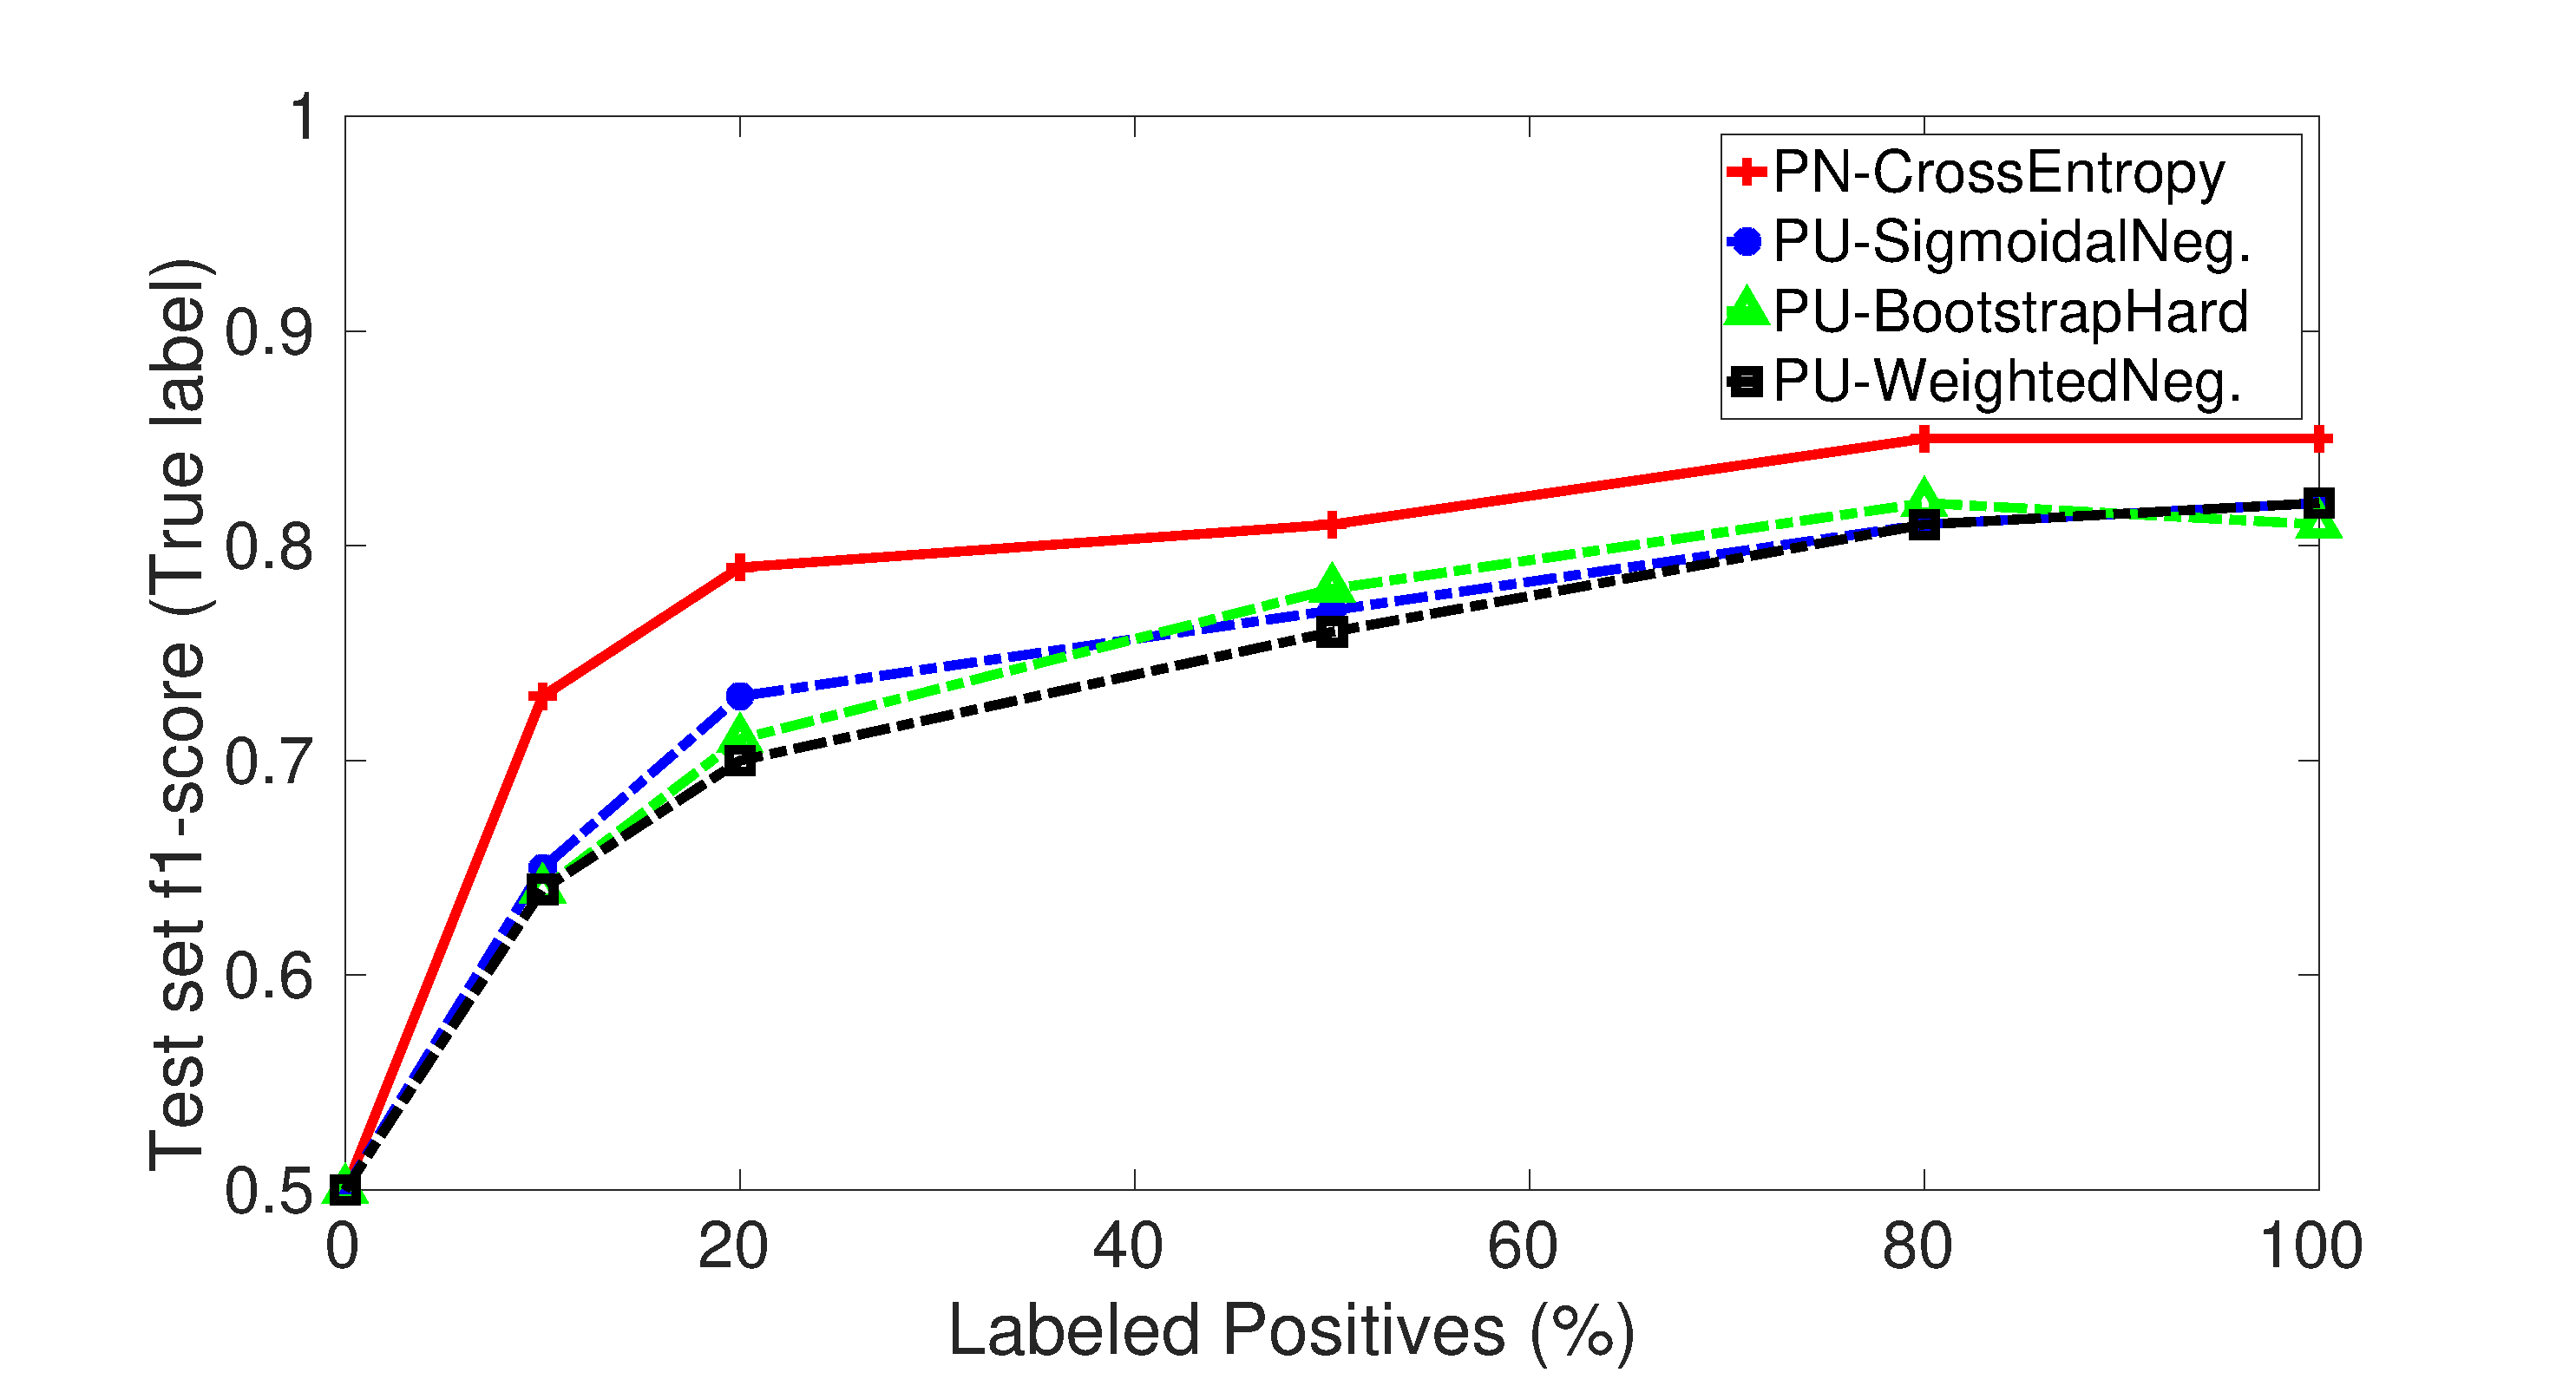
\includegraphics[width=\linewidth]{img/pu_vs_pn}
\caption{Varying percentage of annotated positives 10\%, 20\%, 50\%, 80\% and 100\% with images from CIFAR10 as the positives and images from CIFAR110 as the negatives.}
\label{fig:pct_annotating}
\end{figure}

%%%%%%%% TABLE CIFAR10
\begin{table}[t]
\resizebox{\columnwidth}{!}{
\centering
\begin{tabular}{ll|llll}
Annotation  & Loss & acc. & prec. & rec. & $F_1$ \\
\hline
Complete    & CrossEntropyU.   & 0.87 & 0.88 & 0.82 & 0.85 \\
50\%(P+N)   & CrossEntropyU.   & 0.83 & 0.84 & 0.78 & 0.80 \\
\hline
50\%P+U     & CrossEntropyU.   & 0.66 & 0.94 & 0.39 & 0.50 \\
50\%P+U     & WeightedU.       & 0.78 & 0.75 & 0.75 & 0.76 \\
50\%P+U     & ExponentialU.    & \textbf{0.81} & \textbf{0.85$\pm0.03$} & 0.72$\pm0.03$ & 0.77 \\
50\%P+U     & BootstrapHard    & 0.80 & 0.76 & \textbf{0.81} & \textbf{0.78} \\
\end{tabular}
}
\caption{Image classification with positive examples partially annotated. The complete dataset contains images from CIFAR10 as the \textbf{positive} (P) set and images from CIFAR110 as the \textbf{negative} (N) set. The unannotated positive examples from P set construct the \textbf{unlabeled} (U) set together with the N set. Experiments were repeated three times with random split of P set and U set, and standard deviations were around 0.01 if not explicitly mentioned.}
\end{table}

Training F-1 0.83 vs 0.81

%%%%%%%% TABLE
\begin{table}[t]
\resizebox{\columnwidth}{!}{
\centering
\begin{tabular}{ll|llll}
Annotation  & Loss & pixel acc. & mean acc. & mean IU & f.w. IU \\
\hline
Complete    & CrossEnt.U    &  &  & & \\
50\%P+U     & CrossEnt.U    & & & & \\
50\%P+U     & WeightedU        &  &  & & \\
50\%P+U     & ExponentialU     &  &  & & \\
50\%P+U     & BootstrapHard    &  &  & & \\
\end{tabular}
}
\caption{Image semantic segmentation with images contain single instance only from the PASCAL VOC2011 segmentation dataset. The complete \textbf{positive} (P) set denotes the foreground instances and the \textbf{negative} (N) set consists of the background. The unannotated instances from P set construct the \textbf{unlabeled} (U) set together with the N set.}
\end{table}


\section{Discussion}
\label{sec:discussion}


\paragraph{Binarizing/catergoring classes}
\begin{itemize}
  \item Tradeoff between precise bu inaccurate labels and accurate but inprecise labels
  \item The success of region proposal network is a prove of binarized labels can information about ``objectness''.
  \item Though it may depends on the scale of dataset. But since segmentation dataset is often small, it could be fine.
\end{itemize}

\paragraph{Upsides and downsides of exponential loss}
% Imbalanced
% Easily classified negatives comprise
% the majority of the loss and dominate the gradient. While
% α balances the importance of positive/negative examples, it
% does not differentiate between easy/hard examples
\begin{itemize}
  \item treat easy/hard classifications differently
  \item not over-punish confident positive prediction for negatively labeled examples
  \item easy to implement with the assumption of label noise spatial independence
\end{itemize}


Downside:
\begin{itemize}
  \item Non-parameterizable
  \item Optimization diffilculty introduced as a result of non-convex objective
\end{itemize}


\paragraph{Future works}

\begin{itemize}
  \item Parameterizing exponential unlabeled loss to determine boundaries of confident and unconfident predictions
  \item Take into account label noise spatial dependence for neighboring pixels
  \item Experiment with over-segmentation and under-segmentation noises (negative influence expected)
  \item Experiment with real datasets
\end{itemize}


\section{Conclusion}
\label{sec:conclusion}

We studied how to pre-train transferable convolutional weights in the presence of inexhaustive segmentation, misclassification and false segmentation.
Given that including false segmentations of meaningful objects had little impact on the fine-tuning performance of transferred weights, we proposed to include false segmentation objects to learn the pre-trained model.
By contrast, misclassification noises can have negative impacts on feature transferability, but binarizing classes to foreground and background can produce accurate but not necessarily precise labels to train better transferable features.
We presented that for a small pre-training set, binarizing classes can recover the negative influence of misclassification of object segments on the fine-tuning performance of the transferred models.
Inexhaustive segmentation can also negatively affect feature transferability of the pre-trained model.
The decrease of the fine-tuning performance due to the unsegmented objects in the pre-training set can be compensated by modifying the loss function for deep learning models.
We then proposed a class-dependent loss to not over-punish the confident positive predictions for examples with negative labels.
The proposed sigmoidal negative loss was demonstrated to improve both the pre-training and fine-tuning performance of models pre-trained in the presence of inexhaustive segmentations.



{\small
\bibliographystyle{plain}
\bibliography{references}
}

\clearpage
\appendix


%%%%%%%%%%%%%%%%%%%%%%%%%%%%%%%%%%%%%%%%%%%%%%%%%%%%%%%%%%%%%%%%%%%%%%
%%%%%%%%%%%%%%%% Convolutional Networks for Semantic Segmentation
%%%%%%%%%%%%%%%%%%%%%%%%%%%%%%%%%%%%%%%%%%%%%%%%%%%%%%%%%%%%%%%%%%%%%%

\section{Convolutional Networks for Semantic Segmentation}
\label{sec:cnn4seg}

\subsection{Convolutional Neural Networks}
\label{subsec:cnn}

%%%%%%%% CNN in one sentence

The main components of a typical convolutional neural network (CNN) are several layers of convolutions and sub-sampling, followed by a few fully-connected layers.


%%%%%%%% FIGURE LeNet
\begin{figure}[t]
\centering
   \includegraphics[width=\linewidth]{img/no_padding_no_strides_00.pdf}
\caption{
A basic convolution operation.
A 3x3 convolutional filter convolves with a 3x3 window sliding over the image (bottom).
The output of convolutions at each sliding position form a feature map (top).
This figure was drawn by Dumoulin and Visin \cite{dumoulin2016guide}
}
\label{fig:conv}
\end{figure}

%%%%%%%% LeNet

An example CNN model, LeNet-5 (1998) \cite{lecun1998gradient}, is shown in Figure \ref{fig:lenet}.
The first convolutional layer of LeNet contains 6 convolutional kernels of size 5x5 and each convolutional kernels convolve with small windows sliding over the images and produce a feature map of size 28x28.
Each output in the produced feature map is corresponding to a small sub-region of the visual field (the image), called a \textit{receptive field}.
A following max pooling layer subsamples the feature maps by a factor of two by extracting the maximum values for every two adjacent pixels literally and vertically.
The result feature map S2 has a shape of 14 by 14 and a receptive field of 6 by 6.
Another sequence of convolutional and pooling layers generate feature maps of size 5x5 with receptive field 16x16.
Neurons in the last three layers of LeNet are fully connected to the layer before and the layer after if exists, creating the final prediction for 10 classes.

%%%%%%%% Feature Hierarchy
Features produced by CNN models have a rich hierarchy varying from local to global, from simple to complex.
The bottom layers in the convolutional layer stack have smaller receptive fields and the top layers have larger receptive fields.
A small receptive field means that the filter have access to information only in a local sub-region of the image while a large receptive field can convey more global information.

The various pattern responses from local to global, from simple to complex for stacked convolutional layers is a reflect of emulating animals visual cortex.
In cat's visual cortex \cite{hubel1962receptive}, two basic cell types of visual cortex have been identified:
Simple cells respond maximally to specific edge-like patterns within their receptive field.
Complex cells have larger receptive fields and are locally invariant to the exact position of the pattern.
The shallower convolutional layers play a similar functionlity as simple cells while the deeper layers maps are similar to complex cells.

%%%%%%%% FIGURE LeNet
\begin{figure}[t]
\centering
   \includegraphics[width=\linewidth]{img/lenet}
\caption{An example convolutional neural network, LeNet-5 \cite{lecun1998gradient}}
\label{fig:lenet}
\end{figure}

%%%%%%%% Design of CNN

The main benefit of CNN compared to a standard multilayer neural network (multilayer perceptron) is that
1. take advantage of the 2D structure of an input image
2. it is easier to optimize because of spatial weights sharing and local connectivy pattern of convolutional layers.
Convolutional neurons and maximum pooling, translation invariance as well as scaling invariance and distortion invariance to some extent are achievable for convolutional neural networks. \cite{lecun1998gradient}
Different from the traditional handcrafted features, learnable convolutional features normally generalize well and can achieve better performance for dataset with a complex input distribution. \cite{krizhevsky2012imagenet}
By increasing the number of convolution layers and number of filters in each layer, one can create CNN models with high capacity, meaning a large space of representable functions.
This can be beneficial for datasets of immense complexity, for example, ILSVRC \cite{russakovsky2015imagenet}, Microsoft COCO \cite{lin2014microsoft}, as long as there are sufficient training samples with an appropriate optimization strategy.


\subsection{Semantic image segmentation}
\label{subsec:segmentation}

%%%%%%%% Segmentation in one sentence

Semantic image segmentation is to segment images into semantically meaningful partitions, a.k.a.,\textit{segments}.
It can be operated as classifying pixels into the corresponding pre-defined categories.

%%%%%%%% Difficulty in adapting CNN

CNN models on object classification tasks can be adapted to perform semantic image segmentation tasks. \cite{long2015fully}
One of the primary challenges of applying CNN model to segmentation tasks is how to combine global information and local information to solve semantics and localization altogether.
In contrast to object classification tasks, which normally only need global information to resolve semantics, segmentation tasks also require local information to resolve locations.

%%%%%%%% An example segmentation framework: FCN

Long et al. \cite{long2015fully} proposed a so-called skip architecture in the Fully convovolutional networks (FCN) to aggregate information from the local low-level features in the hierarchy with global information from the high-level features.
As we discussed in the previous session, convolutional layers can extract hierarchical features, varying from low-level to high-level encode information from local to global.
The low-level features are fine, presenting appearances and the high-level features are coarse, revealing semantics.
By combining them together, it becomes possible to create accurate and detailed segmentation.
% in an end-to-end, pixel-by-pixel fully convolutional neural networks for semantic segmentation.

%%%%%%%% FIGURE FCN

\begin{figure}[t]
\centering
   \includegraphics[width=\linewidth]{img/fcn}
\caption{Fully convolutional network (FCN) by Long et al. (2015)  \cite{long2015fully}.
Each }
\label{fig:fcn}
\end{figure}

%%%%%%%% Transferring convolutional neural nets

Convolutional layers in FCN for feature extractions (solid arrows in Figure \ref{fig:fcn}) can be transferred from ImageNet models.


%%%%%%%%%%%%%%%%%%%%%%%%%%%%%%%%%%%%%%%%%%%%%%%%%%%%%%%%%%%%%%%%%%%%%%
%%%%%%%%%%%%%%%% Deep Learning with label noise
%%%%%%%%%%%%%%%%%%%%%%%%%%%%%%%%%%%%%%%%%%%%%%%%%%%%%%%%%%%%%%%%%%%%%%


%%%%%%%% To explain why modifying losses

\section{Cost function and Optimization}

\subsection{Cross entropy loss}
\label{subsec:crossentropy}

The cross entropy loss (a.k.a. softmax loss) is one of the most commonly used cost function for convolutional neural networks in classification problems.
Let $x^{(i)}$ be an input example from totally $m$ examples, $y^{(i)} \in {0,...,K}$ be the corresponding label, and $\theta$ be parameteres of model $f(\cdot)$.
The cross entropy loss is defined as:
$$J(\theta) = - \sum_{i=1}^{m}\sum_{k=0}^{K} 1\{y^{(i)}=k\} \log P(y^{(i)}=k \vert x^{(i)}; \theta)$$
In the equation above, $1\{\cdot\}$ is the ``indicator function'' defined as:
\[
  1\{\text{statement}\} =
    \begin{cases}
      1, & \text{statement is true} \\
      0, & \text{otherwise}
    \end{cases}
\]
$P(y^{(i)} = k | x^{(i)} ; \theta) = \sigma(f(x;\theta))_k$ is the likelihood of $y^{(i)}$ being $k$, predicted by model $f(\cdot)$, where $\sigma(\cdot)_{k}$ is the softmax function that applies to model output for the $k$-th class.

Model outputs $f(x^{(i)};\theta)$ is a vector of $k$ elments with values varying from negative infinity to positive infinity.
Each element of the output vector is corresponding to one class out of $K$ classes.
A larger output value for one class, $k$, than another, $j$, means that the example $x^{(i)}$ is more likely to be class $k$ than class $j$.
The softmax function ensures that the model outputs are normalized to a region between 0 and 1, and sum up to 1 for all classes so that the result outputs fullfils a probability distribution over $K$ different possible outcomes.

The cross entropy loss is a form of negative log-likelihood.
The loss is closed to zero if the predicted probability of $y^{(i)}$ is large, and takes a large positive value if the probability is small.
Minimizing the negative log likelihood of the correct class can be interpreted as performing Maximum Likelihood Estimation (MLE), a commonly optimization.

\subsection{Gradient based optimization and Backpropagation}
\label{subsec:backprop}

The model is optimized by solving the optimal $\theta$ that minimizes the loss function.
It is impossible to solve $\theta$ for a non-linear model analytically so that a gradient-based optimization can be used as an efficient alternative.

The derivative of the cross entropy loss with respect to the $k$-th parameter of the last layer $\theta_k^{(L)}$ is:
\begin{equation*}
  \resizebox{\columnwidth}{!}{
  $ \nabla_{\theta^{(L)}_k} J(\theta) = - \sum_{i=1}^{m}{ \left[ z^{(i)} \left( 1\{ y^{(i)} = k\}  - P(y^{(i)} = k | x^{(i)}; \theta) \right) \right]  } $
  }
\end{equation*}
where the superscription $(L)$ of $\theta$ denotes the layer number of the last layer, and $z^{(i)}$ is the output of the last layer for the $i$-th example.

Weights of the last layer in the $t+1$-th iteration is updated by:
$$\theta_{t+1}^{(L)} = \theta_t^{(L)} - \alpha \nabla_{(\theta^{(L)})} J(\theta)$$
where $\alpha$ is the learning rate determining how quickly the weights are updated.

Gradients in the layers $l<L$ are calculated via a so-called back propagation of errors.
The error of $l$-th layer is propagated the layer after $l+1$:
$$\delta^{(l)} = \left((\theta^{(l)})^T \delta^{(l+1)}\right) \bullet f'(z^{(l)})$$
where $f'(z^{(l)})$ is the derivative of the activation function.
Gradients with respect to weights for the $l$-th layer is:
$$
\nabla_{\theta^{(l)}} J(\theta) = \delta^{(l+1)} (a^{(l)})^T
$$

The weights update for the $l$-th layer in the $t+1$ is computed similarly as the last layer by:
$$\theta_{t+1}^{(l)} = \theta_t^{(l)} - \alpha \nabla_{(\theta^{(l)})} J(\theta)$$

% %
%
% %%%%%%%%%%%%%%%%%%%%%%%%%%%%%%%%%%%%%%%%%%%%%%%%%%%%%%%%%%%%%%%%%%%%%%
% %%%%%%%%%%%%%%%% Deep Learning with label noise
% %%%%%%%%%%%%%%%%%%%%%%%%%%%%%%%%%%%%%%%%%%%%%%%%%%%%%%%%%%%%%%%%%%%%%%
%
% \section{Label noises}
%
% %%%%%%%% To clarify inputs independence and spatial independence of noises
%
% Label noises can be categoried into three statistical models, noisy complete at random (NCAR), noisy at random (NAR) and noisy not at random (NNAR), based on whether label noises depends on classes and distribution of inputs. (Figure \ref{fig:noises})
% For noisy completely at random models, the occurrence of an error $E$ is independent of neither the true class $Y$ nor the input $X$.
% The noisy at random model is similar to the noisy completely at random model except that the label noise is asymmetric, meaning it depends on classes.
% The noisy at random model model can be interpreted in terms of a transition (or confusion) matrix for $K$ classes:
% \[
% \gamma =
% \begin{bmatrix}
%     P(Y^{\ast}=1\vert Y=1)   & \dots  & P(Y^{\ast}=K\vert Y=1) \\
%     \vdots                   & \ddots & \vdots \\
%     P(Y^{\ast}=1\vert Y=K) & \dots  & P(Y^{\ast}=K\vert Y=K)
% \end{bmatrix}
% \]
% where $Y^{\ast}$ is a random variable for observed label and $Y$ true label.
% The noisy not at random, on the other hand, represents that the label noise depends on both class and example.
%
% \begin{figure}[t]
% \begin{center}
% % \fbox{\rule{0pt}{2in} \rule{0.9\linewidth}{0pt}}
%    \includegraphics[width=1.05\linewidth]{img/label_noises}
% \end{center}
%    \caption{
%    Graphical models for three types of label noises. \cite{frenay2014classification}
%    The graphical models describe if the probability of the errorness and observed value of a label conditions on the true class and inputs.
%    $X$ is the random variable denotes the inputs;
%    $Y$ is stands for the variable for class;
%    $E$ is a binary variable determining errorness;
%    $Y^{\ast}$ represents a variable for the observed label;
%    }
% \label{fig:noises}
% \end{figure}
%
% In this thesis, we assumed mislabeling of segmentations is noisy at random. {TODO}



%%%%%%%%%%%%%%%%%%%%%%%%%%%%%%%%%%%%%%%%%%%%%%%%%%%%%%%%%%%%%%%%%%%%%%
%%%%%%%%%%%%%%%% Supportive information
%%%%%%%%%%%%%%%%%%%%%%%%%%%%%%%%%%%%%%%%%%%%%%%%%%%%%%%%%%%%%%%%%%%%%%
\section{Additional information}
\label{sec:support}


\subsection{An 8-layer Convolutional neural network}
\label{subsec:8layer}

The architecture of the 8-layer convolutional neural network used in the classification of CIFAR dataset is presented in Table \ref{tab:8layer}.

% Please add the following required packages to your document preamble:
%%%%%%%% Table 8-layer CNN
\begin{table}[t]
\resizebox{\columnwidth}{!}{
\centering
\begin{tabular}{c|c|c}
\hline
layer name             & output size                     & 8-layer                               \\ \hline
\multirow{3}{*}{conv1} & \multirow{3}{*}{16 $\times$ 16} & 3 $\times$ 3, 32, LeakyReLU(0.2)      \\ \cline{3-3}
                       &                                 & 3 $\times$ 3, 32, LeakyReLU(0.2)      \\ \cline{3-3}
                       &                                 & 2 $\times$ 2 max pool, dropout(0.2)   \\ \hline
\multirow{3}{*}{conv2} & \multirow{3}{*}{8 $\times$ 8}   & 3 $\times$ 3, 64, LeakyReLU(0.2)      \\ \cline{3-3}
                       &                                 & 3 $\times$ 3, 64, LeakyReLU(0.2)      \\ \cline{3-3}
                       &                                 & 2 $\times$ 2 max pool, dropout(0.2)   \\ \hline
\multirow{3}{*}{conv3} & \multirow{3}{*}{4 $\times$ 4}   & 3 $\times$ 3, 128, LeakyReLU(0.2)     \\ \cline{3-3}
                       &                                 & 3 $\times$ 3, 128, LeakyReLU(0.2)     \\ \cline{3-3}
                       &                                 & 2 $\times$ 2 max pool, dropout(0.2)   \\ \hline
\multirow{2}{*}{fc}    & \multirow{2}{*}{1 $\times$ 1}   & flatten, 512-d fc, ReLU, dropout(0.5) \\ \cline{3-3}
                       &                                 & 11-d fc, softmax                      \\ \hline
\multicolumn{2}{c|}{Parameters}                          & 1,341,739                             \\ \hline
\end{tabular}
}
\caption{8-layer Convolutional Neural Networks used in the classification of the CIFAR dataset.}
\label{tab:8layer}
\end{table}

\subsection{Evaluation metrics}

% \noindent (overall) accuracy
$$ \text{accuracy} = \frac{\text{true pos. + true neg.}}{\text{true pos. + false pos. + true neg. + false neg.}}$$

% \noindent precision
$$\text{precision} = \frac{\text{true pos.}}{\text{true pos. + false pos.}}$$

% \noindent recall
$$\text{recall} = \frac{\text{true pos.}}{\text{true pos. + false neg.}}$$

% \noindent f1-score
$$F_1 = 2 \cdot \frac{\text{precision} \cdot \text{recall}}{\text{precision}+\text{recall}}$$

% \noindent intersection over union (IU)
$$ \text{IU} = \frac{\text{true pos.}}{\text{true pos. + false pos. + false neg.}}$$



%%%%%%%%%%%%%%%%%%%%%%%%%%%%%%%%%%%%%%%%%%%%%%%%%%%%%%%%%%%%%%%%%%%%%%
%%%%%%%%%%%%%%%% Appendix Results                     %%%%%%%%%%%%%%%%
%%%%%%%%%%%%%%%%%%%%%%%%%%%%%%%%%%%%%%%%%%%%%%%%%%%%%%%%%%%%%%%%%%%%%%

% \section{Additional Results}
% \label{sec:addition}
%
% %%%%%%%% FIGURE Number of training categories
% \begin{figure}[t]
% \centering
%    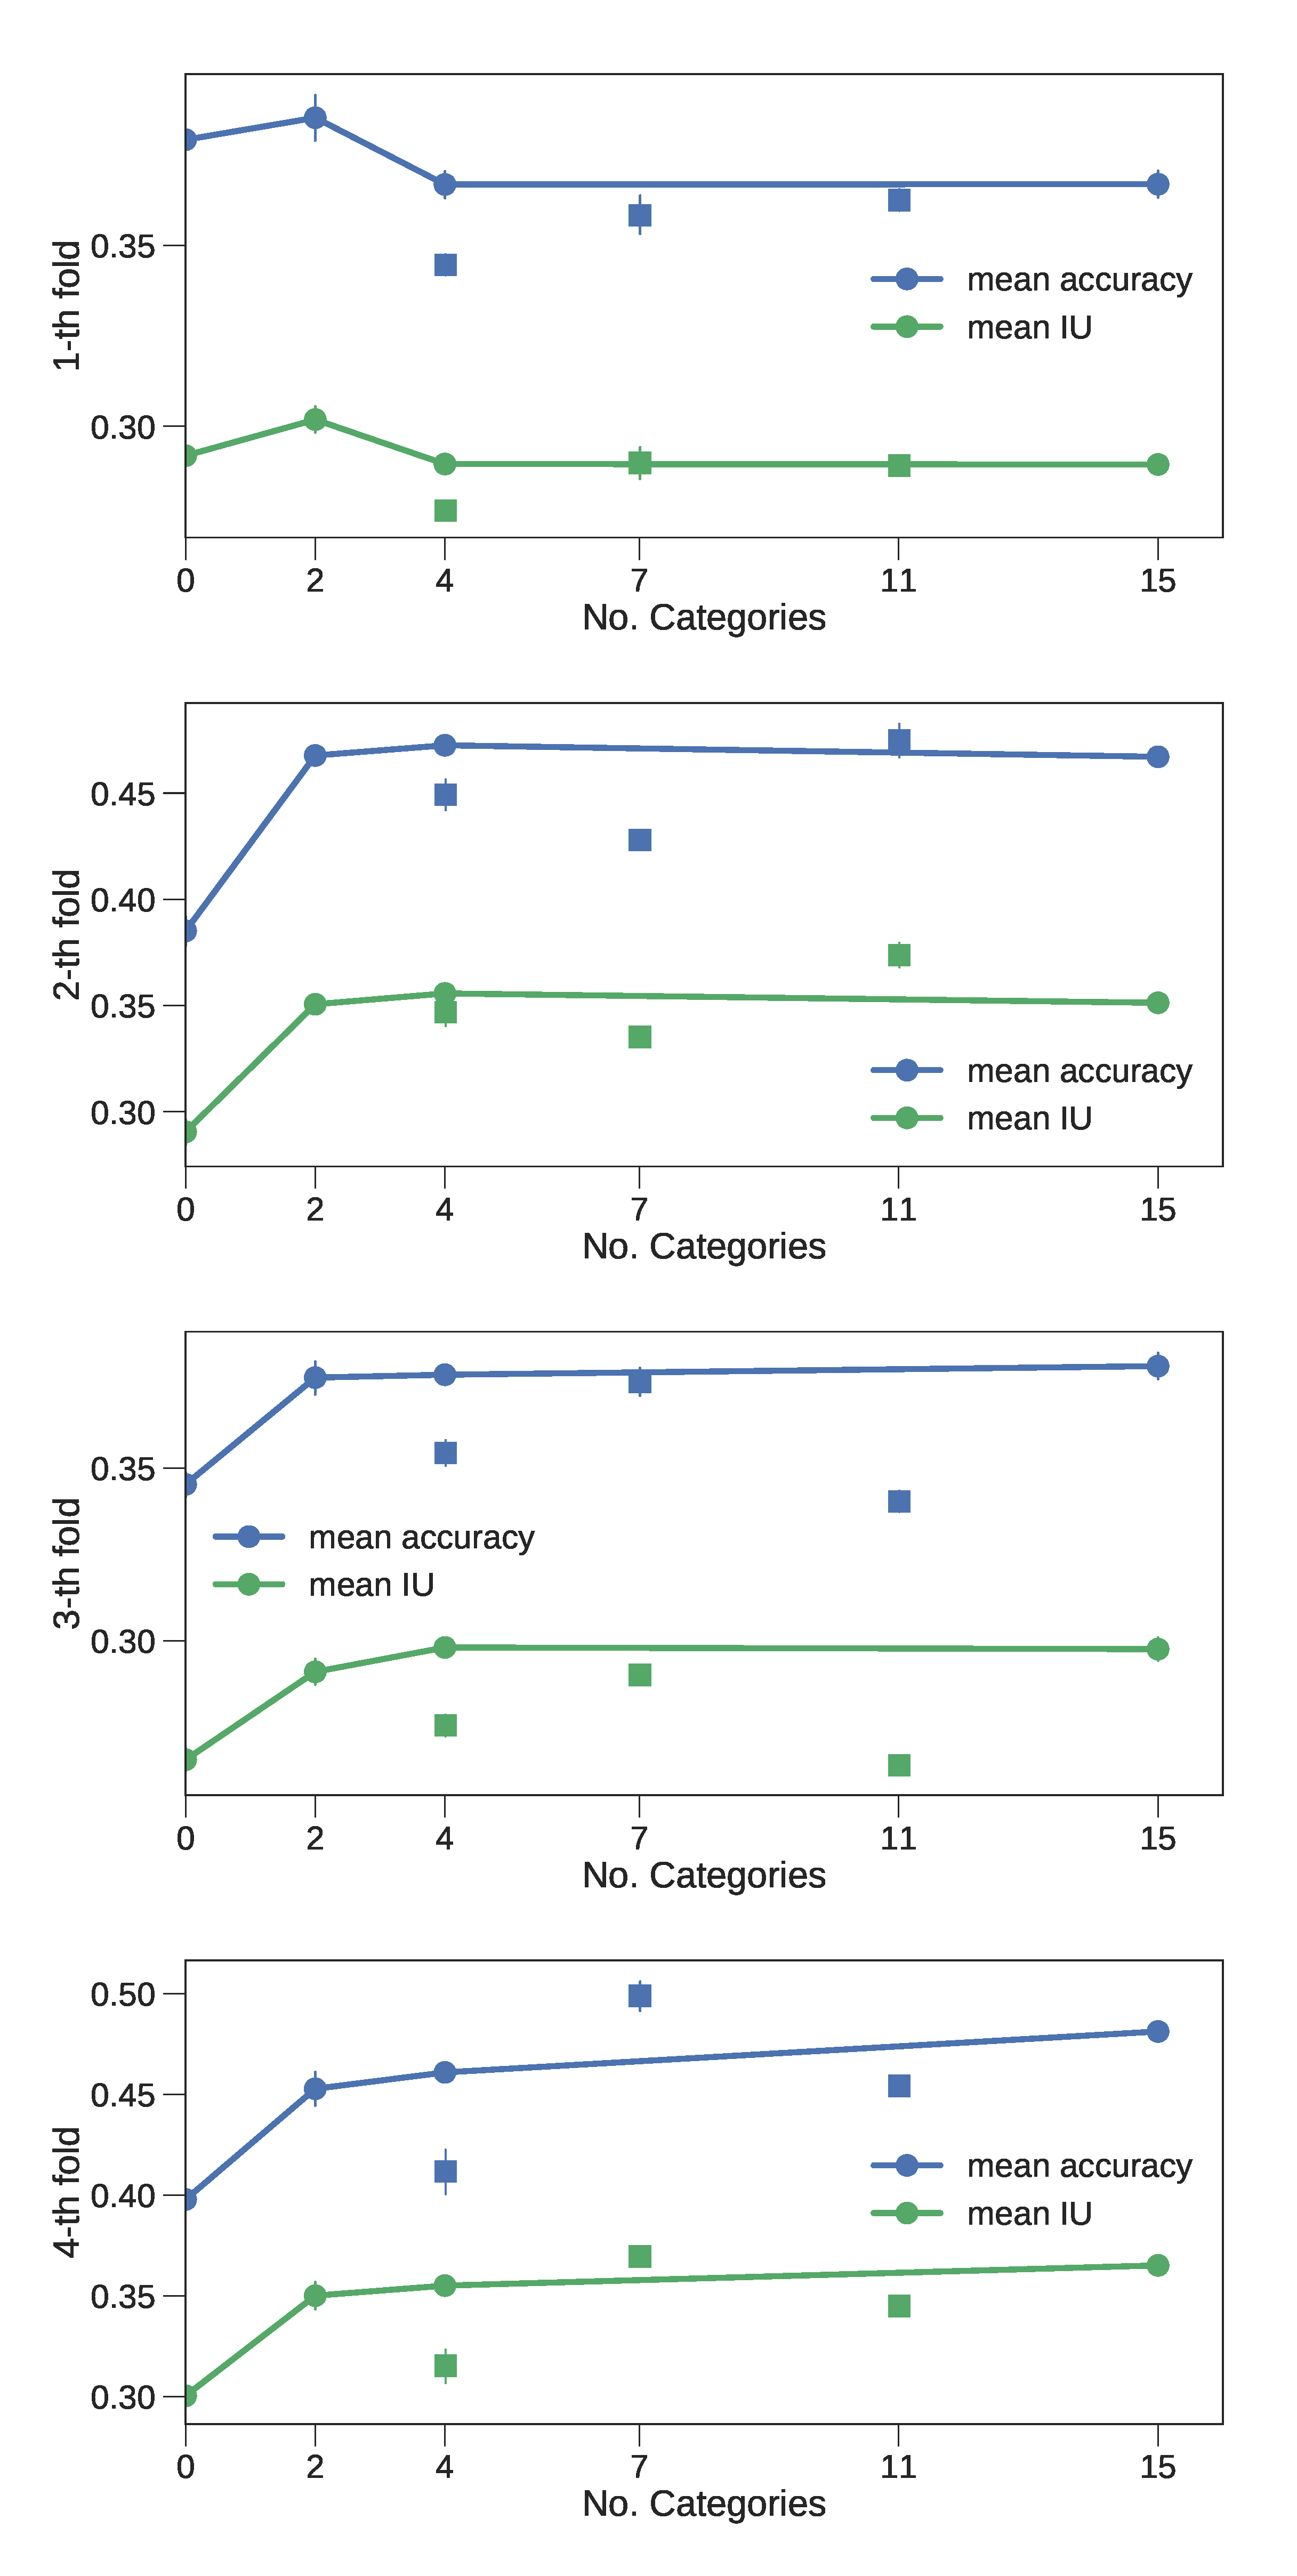
\includegraphics[width=\linewidth]{img/num_classes_folds.eps}
% \caption{The influence of categorizing classes on test performance of fine-tuned models for each fold, addition to Figure \ref{fig:categories}.}
% \label{fig:classesfold}
% \end{figure}


\end{document}
